\documentclass[a4paper, 15pt]{article}
\usepackage[left=0.85in, right=0.85in, top=0.5in, bottom=0.95in]{geometry}
\usepackage[T1]{fontenc}
\usepackage[utf8]{inputenc}
\usepackage[italian]{babel}
\usepackage[none]{hyphenat} % no sillabazione 
\usepackage{multicol} %testo su più colonne
\usepackage{enumerate}
\usepackage{enumitem}
\usepackage{mdwlist} %suspend enumerate \suspend{} \resume{}
\usepackage{lipsum} %testo random per verifica \lipsum
\usepackage{graphicx, nicefrac}
\usepackage{wrapfig2}
\usepackage{amsmath}
\usepackage{mathtools}
\usepackage{amssymb}
\usepackage{amsthm} %teoremi e dimostrazioni e definizioni
\usepackage{cases}
\usepackage{gensymb} %simboli come ° = \degree  etc etc
\usepackage{cancel} %permette di fare semplificazioni utilizzando il comando \cancel{expression}
\usepackage{subcaption}
\usepackage{hyperref}
\hypersetup{
	colorlinks=true,
	linkcolor=blue,    
	urlcolor=blue,
	%pdfpagemode=FullScreen, %il pdf generato non si avvia a schermo intero
}
\urlstyle{same}
\usepackage{changepage}
\usepackage{lastpage, epstopdf}
\usepackage{fancyhdr}
\usepackage{tcolorbox}
%\usepackage{background} %non utilizza lo sfondo con "draft"
\usepackage{color} % testo colorato \textcolor{'ColorCode'}{'testo'}
\usepackage{setspace} % in questo modo posso settare lo spoazio dell'indice \begin{spacing}{0.95}

\usepackage{changepage}
\usepackage{lastpage, epstopdf}
\usepackage{fancyhdr}
\usepackage{tcolorbox}
%\usepackage{background}

%%%%%%%%%%%%%%%%%%%%%%%%%%%%%%%%%%%%%%%%%%%% AMBIENTE TIKZ 
\usepackage{tikz} %disegni e mappe
\usetikzlibrary{patterns}
\usepackage{pgfplots}
\pgfplotsset{compat=1.15}
\usepackage{mathrsfs}
\usetikzlibrary{arrows,decorations.markings,arrows.meta, decorations.text}
\usepackage{circuitikz}

\tikzset{immagine/.style={%
		above right, inner sep=0pt, outer sep=0pt},
	testo/.style={fill=white, align=center,
		fill opacity=0.6, text opacity=1, below,
		font=\sffamily\bfseries\footnotesize}}
	
\raggedbottom
\setlength{\parindent}{0pt}
%%%%%%%%%%%%%%%%%%%%%%%%%%%%%%%%%%%%%%%%%%%% SIUNITX 
\usepackage{siunitx}

%========TEOREMI========%
\newtheorem*{thm}{Teorema}
\newtheorem*{en}{Enunciato}
\newtheorem*{definizione}{Definizione}
\newtheorem*{cor}{Corollario}
	
	
	
%========OPERATORI&COMANDI========%
\DeclareMathOperator{\rk}{rk}
\DeclareMathOperator{\im}{Im}
\DeclareUnicodeCharacter{20AC}{\EUR}
\newcommand{\cmark}{\ding{51}}
\newcommand{\xmark}{\ding{55}}
\newcommand{\compresslist}{ % Define a command to reduce spacing within itemize/enumerate environments, this is used right after \begin{itemize} or \begin{enumerate}
				\setlength{\itemsep}{1pt}
				\setlength{\parskip}{0pt}
				\setlength{\parsep}{0pt}
			}
\newcommand{\ra}[1]{\renewcommand{\arraystretch}{#1}} %stretcho le tabelle
			
%\renewcommand{\arraystretch}{2.5} % Da copiaincollare prima di ambienti array per ampliarli un po'
%\setlength{\jot}{10pt} % affecting the line spacing in the environment SPLIT
			
\begin{document}
\setcounterpageref{secnumdepth}{0}	% NON NUMERO I CAPITOLI
\setcounter{tocdepth}{5} % INCLUDO addirittura I sotto-PARAGRAFI
\tableofcontents 
\newpage

\part{5.AMPLIFICATORI OPERAZIONALI}
\section{Introduzione}	
\begin{adjustwidth}{2in}{}
		Gli amplificatori operazionali sono blocchi di misura che si aggiungono al sensore già noto e prendono il nome di manipolatori di segnale, a questi potrà poi seguire un convertitore analogico/digitale a cui seguirà la visualizzazione del segnale tramite PC, USB \dots		
		\begin{figure}[H]
			\centering
			\begin{tikzpicture} [>=latex]
				%\draw[help lines] (0,0)	grid (15,5);		
				\draw[->] (0,2) -- (1,2)  node [pos = 0, left] {x};
				\node[draw] at (2,2) {sensore};
				\draw[->] (3,2) -- (4,2)  node [pos = 0.5, below] {y};
				\node[draw] at (5.5,2) {manipolatore};
				\draw[->] (7,2) -- (8,2)  node [pos = 0.5, below] {y'};
				\node[draw] at (9.5,2) {convertitore};
				\draw[->] (11,2) -- (12,2)  node [pos = 1, right] {out};
			\end{tikzpicture}
		\end{figure}		
		Il blocco di manipolazione del segnale ne permette:
		\begin{itemize}
			\item L'amplificazione;
			\item Il filtraggio;
			\item L'integrazione o la derivazione;
			\item La somma o sottrazione di segnali provenienti da più sensori ;
		\end{itemize}
	
		Quali sono i circuiti elettronici che permetto Queste operazioni? Per eseguirle si necessita di un componente elettronico detto Amplificatore Operazionale, di cui in questa trattazione verrà fornita una spiegazione da utilizzatore. \newline 
		
		L'amplificatore operazionale è un elemento attivo, per cui per funzionare ha bisogno di corrente, solitamente lavora ad una tensione di alimentazione di $\pm15 V$	
\begin{figure}[H]
	\centering
	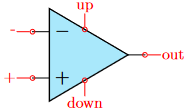
\includegraphics[width=0.3\linewidth]{immagini/screenshot001}
	\label{fig:screenshot001}
\end{figure}
		È perciò caratterizzato da un morsetto negativo chiamato \textit{ingresso invertente}, uno positivo chiamato \textit{ingresso non invertente}, e uno di uscita; oltre a due morsetti di alimentazione. Il morsetto invertente produrrà in uscita un segnale di segno opposto al segnale in ingresso mentre quello non invertente produrrà un segnale nello stesso segno di quello di ingresso, la tensione in uscita è tale che:
		\[V_{out} = A(V_+-V_-)\]
		In cui $A = 10^6 \div 10^9$ è il guadagno; $R_{in} = (10^6\div10^9) \Omega$; $R_{out} =(10\div100) \Omega $. Si ricordi poi come essendo la misura di $V$ una differenza, la $V_{out}$, l'uscita andrà riferita a terra, al ground.  		
\begin{figure}[H]
	\centering
	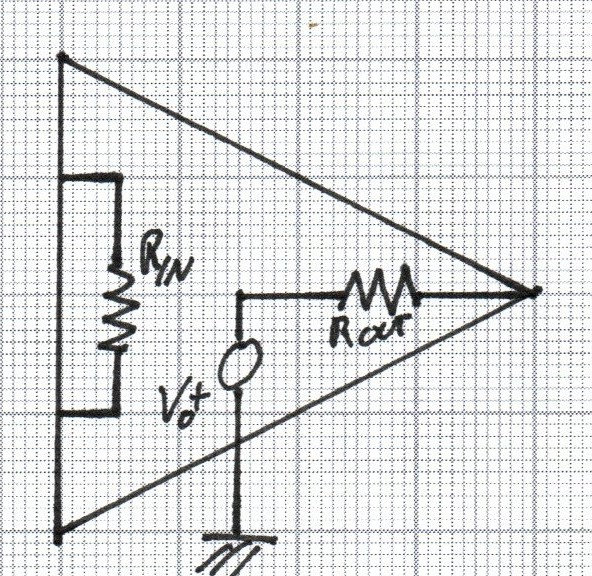
\includegraphics[width=0.2\linewidth]{immagini/mm(1)}
	\label{fig:mm1}
\end{figure}
		Cos'era l'errore di inserzione? Ricordi il termometro nella tazzina? La misurazione, lo strumento di misurazione interferisce col misurando, questo errore è ovviamente present anche nelle misure di tensione. 
		
		Ad esempio si voglia misurare la tensione $V_g$ ai capi di questo circuito, in cui $R_g$ è la resistenza interna del sensore. Un multimetro ideale misurerebbe $V_{ID} = V_g$.		
\begin{figure}[H]
	\centering
	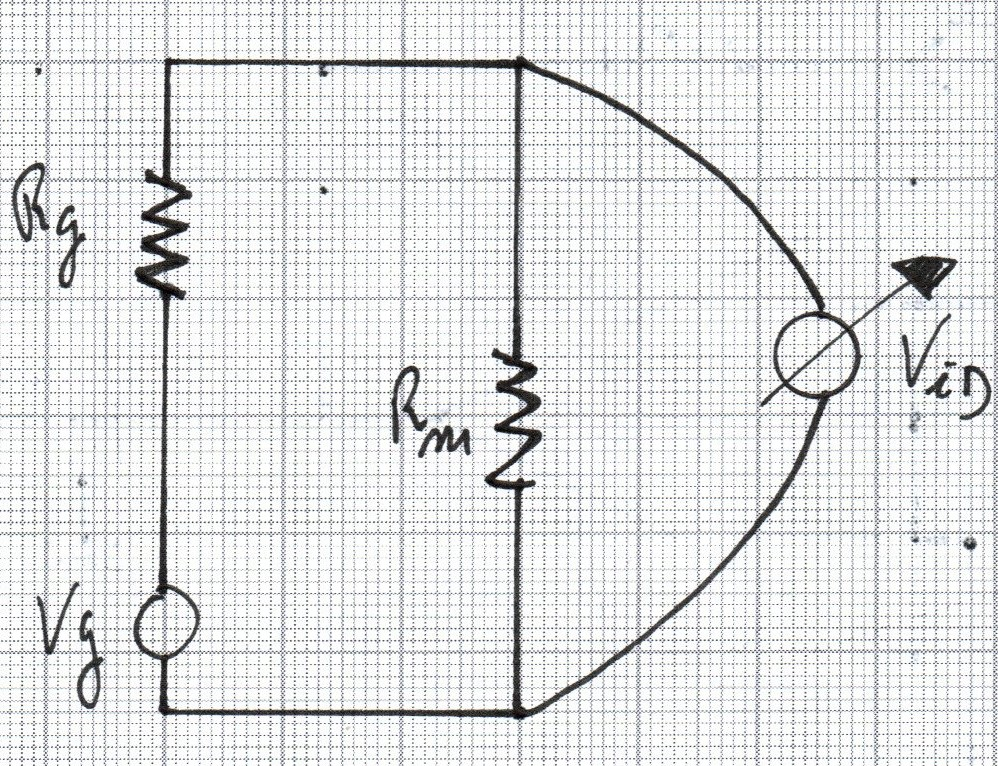
\includegraphics[width=0.2\linewidth]{immagini/mm(2)}
	\label{fig:mm2}
\end{figure}		
		In realtà il multimetro possiede una sua resistenza interna $R_m$, sulla quale scorrerà corrente e porterà errore di inserzione. 				
		\[\begin{dcases}
			V_{Reale} = IR_m \\
			V_g = I(R_g + R_m)
   		\end{dcases} \Rightarrow V_R = \dfrac{R_m}{R_g + R_m}V_g \]
   		Per cui, senza eseguire passaggi già fatti precedentemente:
   		\[\varepsilon_{ins} = \dfrac{V_{ID}-V_R}{V_R} = {R_g\over R_m} \Rightarrow \varepsilon_{ins} \rightarrow 0 ~ \text{se} ~ \begin{cases}
   			R_g\rightarrow0\\
   			R_m\rightarrow\infty
   		\end{cases}\]
   		Magari lo strumento presenta sia un $R_g$ molto alto che un $R_m$ molto basso, come lo si può minimizzare? Inserendo un amplificatore operazionale. 
\begin{figure}[H]
	\centering
	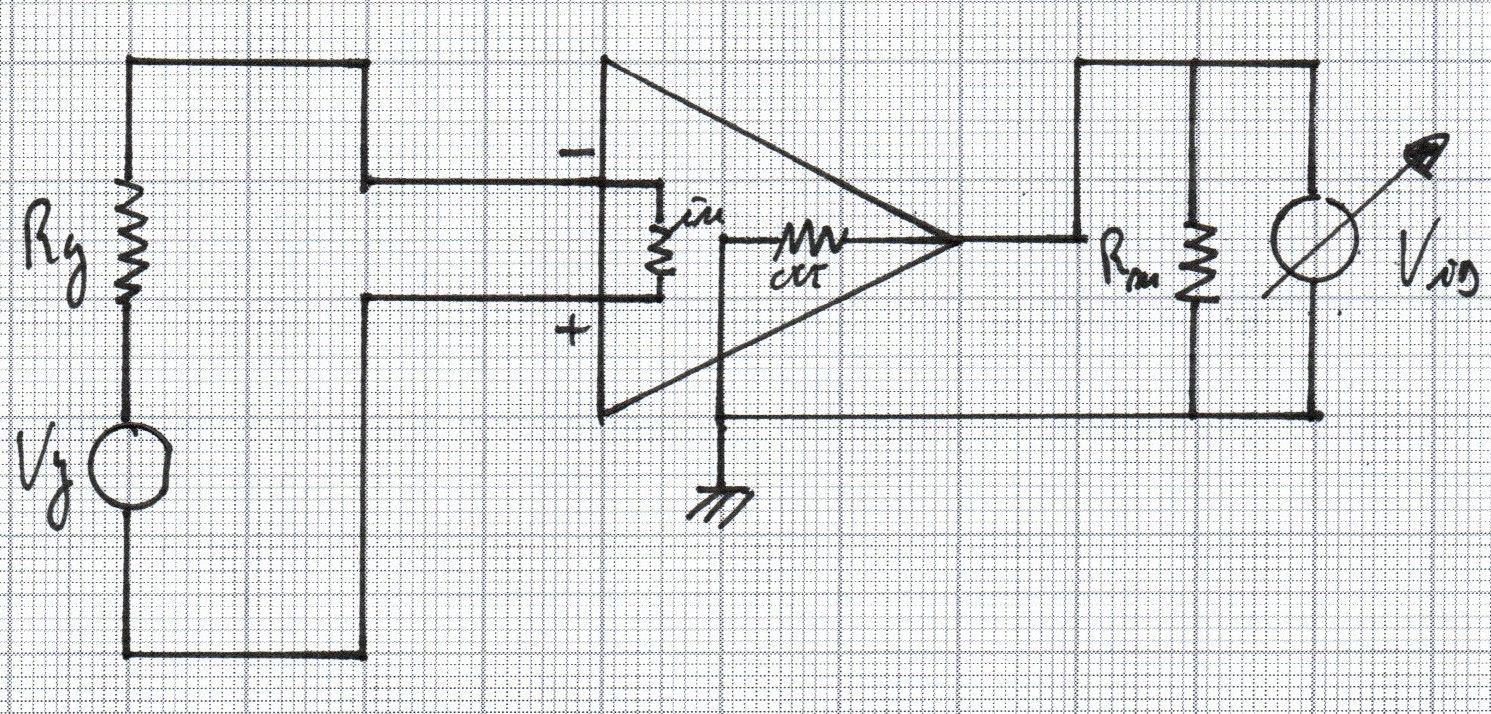
\includegraphics[width=0.3\linewidth]{immagini/mm(3)}
	\label{fig:mm3}
\end{figure}
   		A prima vista potrebbe sembrare di star peggiorando la situazione perché si stanno inserendo due errori di inserzione, un in ingresso all'amplificatore ed uno in uscita:   		
   		\[ \varepsilon_{ins} = \frac{\text{Resistenza da dove viene il segnale}}{\text{Resistenza che vede il segnale}} \hspace{0.5cm} \varepsilon_{ins, in} = {R_g\over R_in} \hspace{0.5cm} \varepsilon_{ins, out} = {R_{out}\over R_m}\]
   		Poiché si è detto che $R_{in}\rightarrow10^9$ e che $R_{out}\rightarrow10$, entrambi gli errori risultano trascurabili: si è notevolmente abbattuto l'errore di inserzione. \newline 
   		
   		In questo caso l'amplificatore operazionale si chiama disaccoppiatore di segnale, disaccoppia il segnale ma va a diminuire l'errore di inserzione. \newline 
   		
   		Ci sono poi altri due utilizzi dell'amplificatore operazionale, in \textbf{Circuito aperto} o in \textbf{Circuito chiuso}.
   		
   		il \textbf{circuito aperto} collega due segnali ed identifica un'uscita: \[V_{out} = A(V_+-V_-)\].  
\begin{figure}[H]
	\centering
	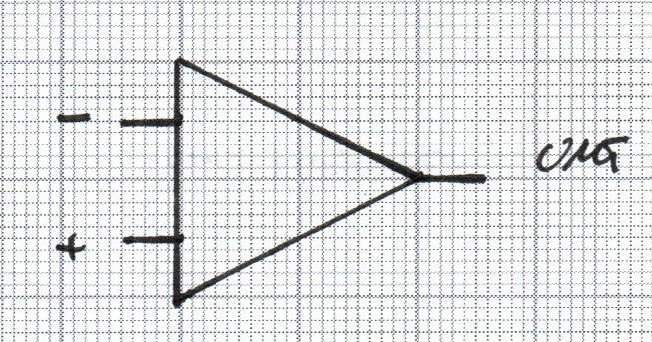
\includegraphics[width=0.2\linewidth]{immagini/mm(4)}
	\label{fig:mm4}
\end{figure}   		
   		Il \textbf{circuito chiuso} o ramo di feedback collega due segnali e si ricollega attraverso un banco di impedenze al ramo negativo.
   		\begin{figure}[H]
   			\centering
   			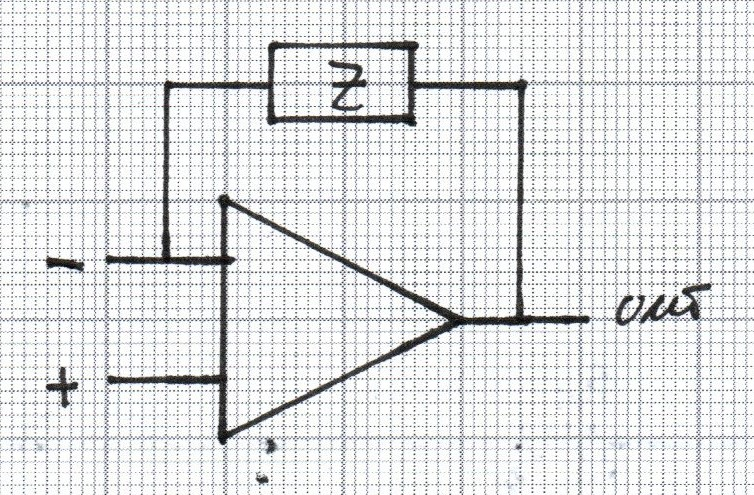
\includegraphics[width=0.2\linewidth]{immagini/mm(5)}
   			\label{fig:mm5}
   		\end{figure}
\end{adjustwidth}
%\newpage
\subsection{Circuito aperto}
\begin{adjustwidth}{2in}{}		
		Per un amplificatore a circuito aperto si può scrivere
		\[V_{out} = A(V_+-V_-)\]
		In questo tipo di amplificatori il guadagno può raggiungere valori dell'ordine di $A = \num{e6}$, poiché il guadagno indica la pendenza della caratteristica ingresso - uscita, più il guadagno cresce più la retta diviene pendente, ciò significa avere una zona di linearità enormemente ridotta.
		\begin{figure}[H]
			\centering
			\subfloat{\begin{circuitikz} \draw
					(0,0) node[op amp] (opamp) {}
					(opamp.+) node[left] {$V_+$}
					(opamp.-) node[left] {$V_-$}
					(opamp.out) node[right] {$V_{out}$}
					(opamp.up) --++(0,0.5) node[vcc]{\textnormal{$V_{cc+}$}}
					(opamp.down) --++(0,-0.5) node[vee]{\textnormal{$V_{cc-}$}}
					;
			\end{circuitikz}} \quad \subfloat{\scalebox{0.6}{\begin{tikzpicture} 
						%\draw [help lines] (0,0) grid (10,10);
						\draw [->](5,0) -- (5,10) node [pos=1, left] {$V_{out}$};
						\draw [->](0,5) -- (10,5) node [pos=1, below] {$V_+-V_-$};
						\draw (5.2,9) -- (4.8,1) node[pos=0.75, left] {$A$};
						\draw (5.2,9) -- (10,9);
						\draw (4.8,1) -- (0,1);
						%Valori 
						\draw[dashed] (5,9) -- (8,9) node[pos=0, left] {$V_{Al}$};
						\draw[dashed] (5.2,5) -- (5.2,9);
						\node at (5.5,4.6) {$V_{Lin}$};
						\node [draw] at (7.5,2.5) {{\footnotesize Circuito aperto}};
			\end{tikzpicture}}}
		\end{figure}
		Infatti per un circuito aperto varrebbe 
		\[\Delta V_{Lin} = \dfrac{V_{cc}}{A} = \SI{15}{\micro\volt}\] 
		Ciò significa che non appena la differenza di tensione in ingresso è di pochissimo superiore allo zero, il segnale satura alla tensione di alimentazione: è per questo che il circuito aperto non può essere usato come amplificatore (tuttalpiù come comparatore), proprio a causa del suo elevatissimo guadagno che limita fortemente la sua zona di linearità.
   		\[\begin{dcases}
   			V_+>V_- \Rightarrow V_{out} = +15 V \\
   			V_+<V_- \Rightarrow V_{out} = -15 V \\
   		\end{dcases}\]   		
   		Notare come non si sta affatto amplificando il segnale, il segnale che si vorrebbe amplificato è quello tratteggiato: si dice quindi che in questo caso l'amplificatore operazionale sta lavorando come un comparatore, Compara due segnali, quando è collegato si saprà quando $V_+>V_-$ e $V_+<V_-$. 
\end{adjustwidth}
\newpage
\subsection{Circuito chiuso}
\begin{adjustwidth}{2in}{}	   		
		Al fine perciò di realizzare un amplificatore che permetta la corretta visualizzazione del segnale amplificato si decide di chiudere il circuito e applicare una retroazione: il segnale in uscita viene riportato all'ingresso mediante un ramo di feedback costituito da elementi passivi, che sebbene comporti un abbassamento del guadagno, permette di avere una zona di linearità maggiore, pur non eliminando del tutto il problema della saturazione.\newline
		
   		Il circuito chiuso si suddivide a sua volta in due configurazioni.  
\begin{itemize}	   		
   		\item \textbf{Invertente}
   		 
   		Il segnale da misurare è collegato al morsetto invertente.   		
   		\begin{figure}[H]
   			\centering
   			\scalebox{0.8}{\begin{circuitikz}
   					%\draw [help lines] (0,0) grid (10,10);			
   					\draw (5,1) node[op amp, anchor=+] (OA1) {};    % Amplificatore
   					\draw (OA1.+) -- (5,-0.5) node[ground]{};       % Ramo non invertente a terra
   					\draw (OA1.-) to [R, l_=$R_i$] (3,2) to[european voltage source, l_=$V_i$] (3,0) -- (3,-0.5) node[ground]{}; % Ramo invertente col segnale
   					\draw (OA1.-) -- (5,3) to [generic, l^=$z$] (5,3 -| OA1.out) -- (OA1.out); % Ramo di feedback
   					\draw (7.5,1) -- (7.5,-0.5) node[ground]{$V_{out}$};	% Uscita		
   			\end{circuitikz}}
   		\end{figure}
   		
   		\item \textbf{Non invertente} 
   		
   		Il segnale da misurare è collegato al morsetto non invertente.    		
   		   		\begin{figure}[H]
   			\centering
   			\scalebox{0.8}{\begin{circuitikz}
   					%\draw [help lines] (0,0) grid (10,10);			
   					\draw (5,1) node[op amp, anchor=+] (OA1) {};    % Amplificatore
   					\draw (OA1.+) to[european voltage source, l_=$V_i$] (5,-0.5) node[ground]{};       % Ramo non invertente a terra
   					\draw (OA1.-) to [R, l_=$R_i$] (3,2) to [short] (3,-0.5) node[ground]{}; % Ramo invertente col segnale
   					\draw (OA1.-) -- (5,3) to [generic, l=$z$] (5,3 -| OA1.out) -- (OA1.out); % Ramo di feedback
   					\draw (7.5,1) -- (7.5,-0.5) node[ground]{$V_{out}$};	% Uscita		
   			\end{circuitikz}}
   		\end{figure}   		
\end{itemize}
\end{adjustwidth}
\newpage
\section{Circuito Chiuso Invertente}
\begin{adjustwidth}{2in}{}	
   		Sul ramo di feedback è posta una resistenza $R_f$.   		
   		\begin{figure}[H]
   			\centering
   			\scalebox{1.5}{\begin{circuitikz}
   					%\draw [help lines] (0,0) grid (10,10);			
   					\draw (5,1) node[op amp, anchor=+] (OA1) {};    % Amplificatore
   					\draw (OA1.+) -- (5,-0.5) node[ground]{};       % Ramo non invertente a terra
   					\draw (OA1.-) to [R, l_=$R_i$] (3,2) to[european voltage source, l_=$V_i$] (3,0) -- (3,-0.5) node[ground]{}; % Ramo invertente col segnale
   					\draw (OA1.-) -- (5,3) to [R, l^=$R_f$] (5,3 -| OA1.out) -- (OA1.out); % Ramo di feedback
   					\draw (7.5,1) -- (7.5,-0.5) node[ground]{$V_{out}$};	% Uscita		
   			\end{circuitikz}}
   		\end{figure}   		
   		\textbf{Principio di massa virtuale}, di Virtual Ground: in prima approssimazione \[V_+ = V_-\].    		
   		Considerazioni:
   		\begin{enumerate}
   			\item \(R_{in}\uparrow \Rightarrow \begin{cases}
   				I\downarrow \approx 0\\
   				\Delta V\downarrow \approx 0
   			\end{cases} \Rightarrow V_+\approx V_-\)
   			\item Dato che il segnale NON satura, si vede segnale in uscita, dalla relazione \(V_{out} = A(V_+-V_-)\) se $A\rightarrow\infty \Rightarrow \Delta V\rightarrow0$ e dunque \(V_+\approx V_-\)
   		\end{enumerate}  	
   		Ora, nel circuito chiuso invertente $V_+=0$ perché è collegato a terra, applicando quindi il principio di massa virtuale si conclude che:
   		\[V_- = V_+ = 0\]
   		E quei morsetti collassano in un nodo, perciò essendo:
   		\[I^* = {V_i-V_-\over R_i} \hspace{1cm} I^{**} = {V_--V_{out}\over R_f} \]
   		Poiché la corrente sul circuito è la stessa, questi di contribuiti devono essere uguali, si ricava così: 
   		\[V_{out} = -{R_f\over R_i}V_i\]
   		In cui ${R_f\over R_i}$ rappresenta il guadagno: si sta amplificando il segnale e lo si sta cambiando di segno, d'altro canto è invertente. \newline 
   		
   		Come amplificare di 5 volte il segnale? Il guadagno dev'essere pari a 5, si scelgono così $R_i = 1k\Omega$ e $R_f = 5k\Omega$.
   		
   		Si ricordi poi che raggiunta la tensione di alimentazione l'amplificatore andrà in saturazione.
   		
   		Disegno grafico fatto bene 
   		
   		NB: Alcune volte amplifica, anche volte non legge neanche il segnale, in dipendenza della tensione di alimentazione (CAPISCI PERCHÉ). 
   		
   		Si può anche deamplificare il segnale, sempre scegliendo opportune resistenze come $R_i = 2k\Omega$ e $R_f = 1k\Omega$.\newline 
\end{adjustwidth}
\newpage
\subsection{Circuito Chiuso invertente sommatore}
\begin{adjustwidth}{2in}{}   	
\begin{figure}[H]
	\centering
	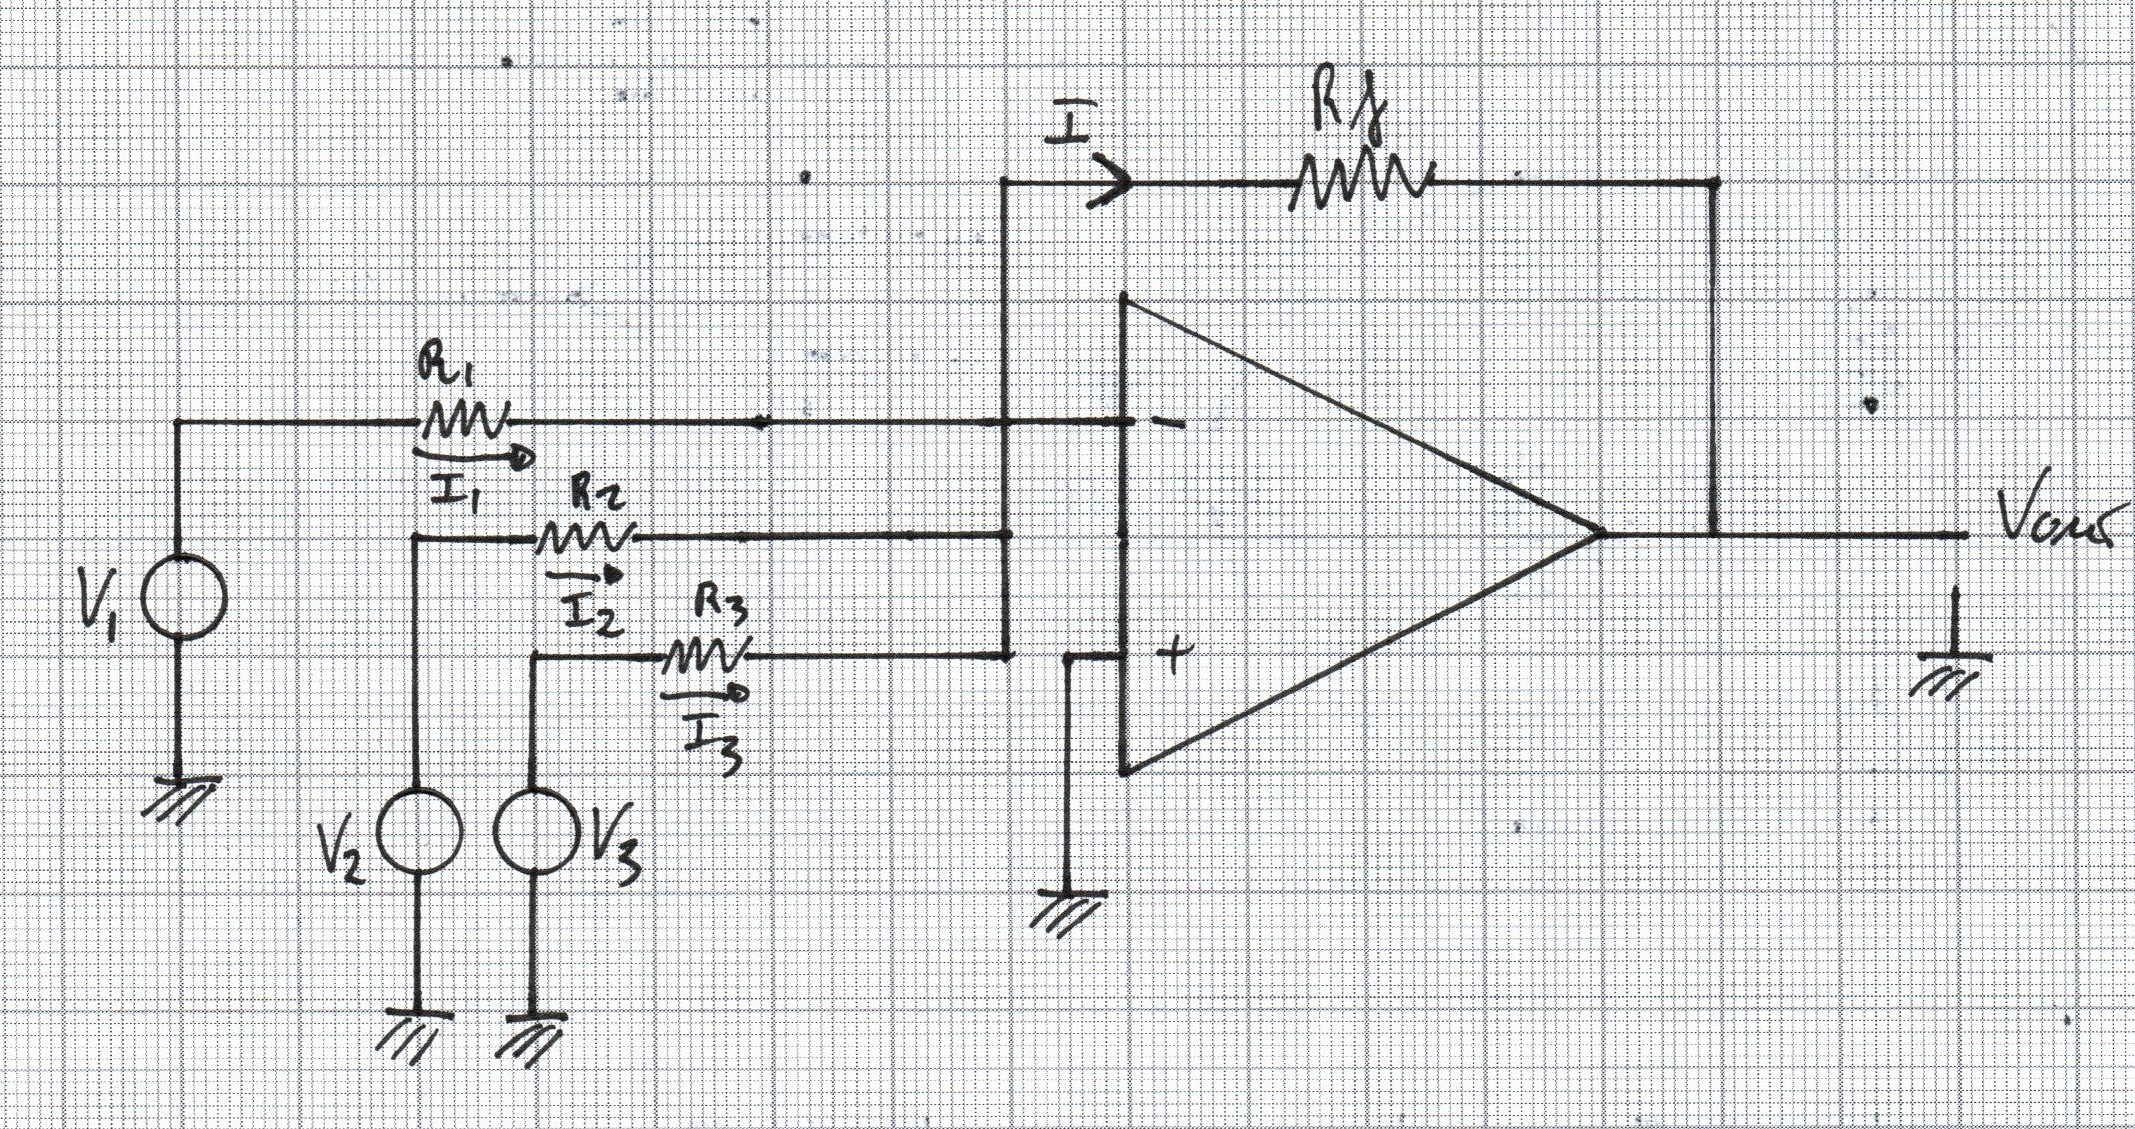
\includegraphics[width=0.5\linewidth]{immagini/mm(6)}
	\label{fig:mm6}
\end{figure}   		
   		Sempre secondo il Principio di massa virtuale \(V_- = V_+ = 0\). 
   		
   		Semplicemente si ha
   		\[I = I_1 + I_2 + I_3 = {V_1\over R_1} + {V_2\over R_2} + {V_3\over R_3} = -{V_{out}\over R_f} \]
   		Allora si ottiene:
   		\[ V_{out} = -R_f\left({V_1\over R_1} + {V_2\over R_2} + {V_3\over R_3}\right) \]
   		Come si ottiene la somma di tre segnali? Scegliendo $R_1 = R_2 = R_3 = R_f$, in questo modo: 
   		\[ V_{out} = -\cancel{R_f}\left({V_1\over \cancel{R_1}} + {V_2\over \cancel{R_2}} + {V_3\over \cancel{R_3}}\right) = -(V_1 + V_2 + V_3) \]
   		
   		E per un \textbf{Circuito mediatore?}, in questo caso si sceglierà $R_1 = R_2 = R_3 = 3R_f$:
   		\[ V_{out} = {-(V_1 + V_2 + V_3)\over3} \]
\end{adjustwidth}
\newpage
\subsection{Circuito Chiuso invertente integratore}
\begin{adjustwidth}{2in}{}    		
   		Questo circuito integra un segnale.
\begin{figure}[H]
	\centering
	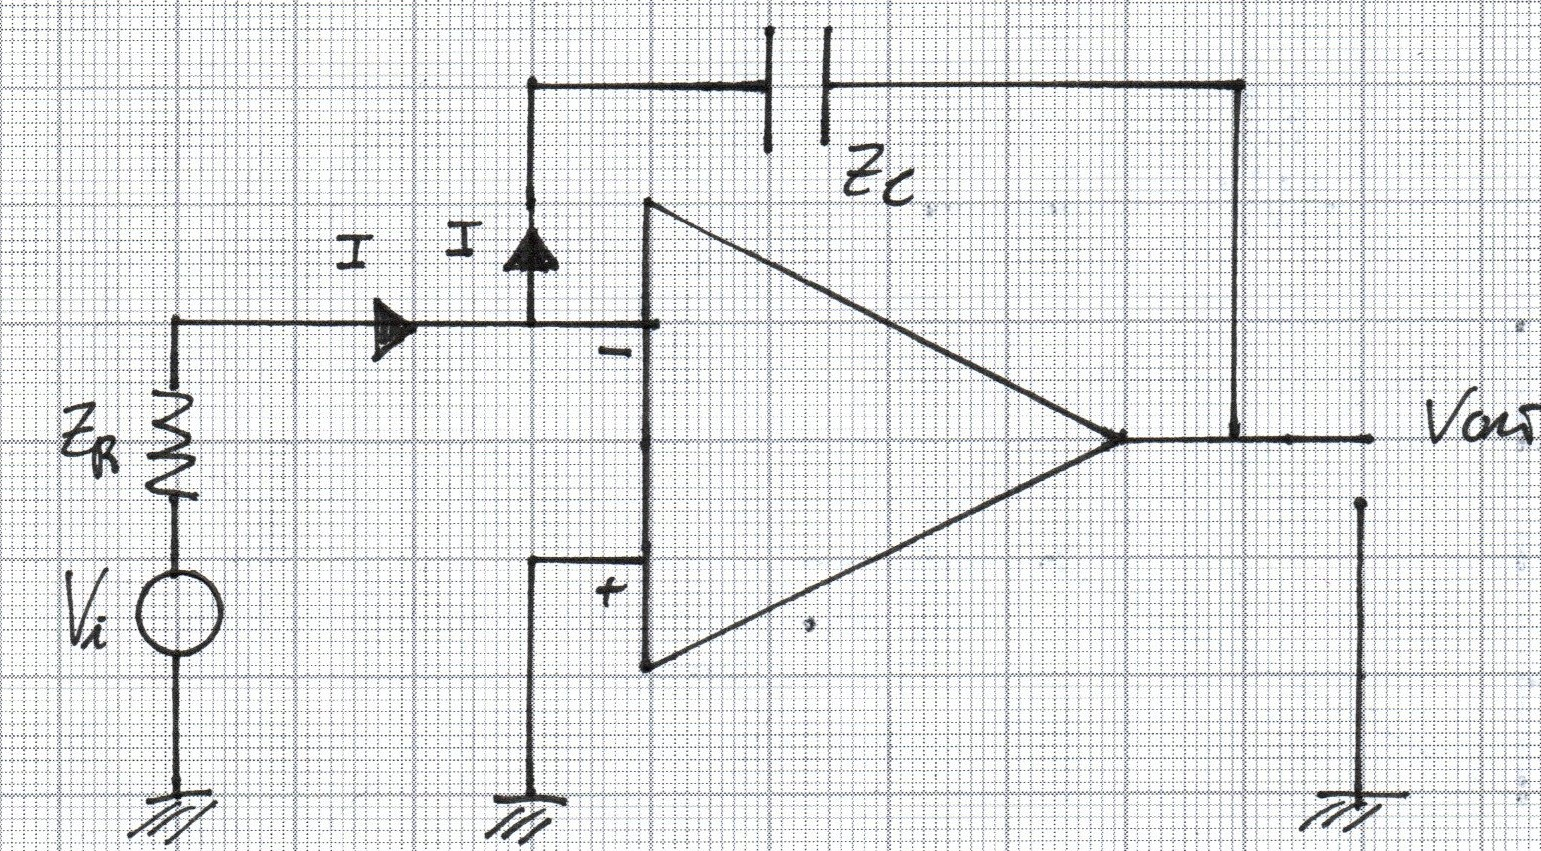
\includegraphics[width=0.5\linewidth]{immagini/mm(8)}
	\label{fig:mm8}
\end{figure}   		
   		Passando attraverso le impedenze: \(Z_R = R_1; Z_C = {1/j\omega C}\), ricordando la relazione che lega ingresso  uscita di un amplificatore si ha:
   		\[{V_{i}\over R_i} = I = -{V_{out\over Z_C}} \Rightarrow V_{out} = -{Z_C\over R_i}V_i = - {1\over j\omega R_iC}V_i\]
   		Esprimendo la tensione di entrata in termini fasoriali questa è: 
   		\[V_i = V_0e^{j\omega t}\]
   		L'integrale di questa tensioni in ingresso è pari a:
   		\begin{eqnarray*}
   			\int V_idt = {V_0\over j\omega t}e^{j\omega t} = {1\over j\omega}V_i  \\
   			\int V_idt = {1\over j\omega}V_i \\
   			V_i = j\omega\int V_idt
   		\end{eqnarray*}
   		Per cui: 
   		\begin{eqnarray*} 
   			V_{out} = - {1\over j\omega R_iC}j\omega\int V_idt = -{1\over R_iC}\int V_idt \\
   			V_{out} = -{1\over R_iC}\int V_idt
   		\end{eqnarray*}
   		Si ottiene così in uscita un segnale integrato. \newline 
   		
   		Il guadagno dell'uscita rispetto all'ingresso è: 
   		\[ G = \left|V_{out}\over V_i\right| = {1\over\omega R_iC}\]
   		Che evidenzia un andamento teorico del genere
   		\begin{figure}[H]
   			\centering
   			\begin{tikzpicture}
   			\begin{axis}[
   				axis lines = left,
   				xlabel = \(\omega\),
   				ylabel = {\(G\)},
   				xticklabels=\empty,yticklabels=\empty]
   				\addplot [domain=0:10, 
   				samples=100, line width=1pt
   				] {
   					1/x
   				};
   			\end{axis}
   		\end{tikzpicture}
   		\end{figure}   		
   		Ricordando sempre che al massimo l'amplificatore raggiunge la tensione di alimentazione, non ottiene mai quel guadagno teorico per le frequenze che tendono a zero. \newline 
   		
   		Quindi cos'è che si ottiene dal circuito invertente integratore? Ad esempio se in ingresso si ha una funzione sinusoidale, questa verrà integrata fornendo in uscita una funzione cosinusoidale leggermente amplificata magari, cambiata di segno, sia ad esempio $IN = \sin(x) \Rightarrow OUT = -1.3(-\cos(x))$. 
   		\begin{figure}[H]
   			\centering
   			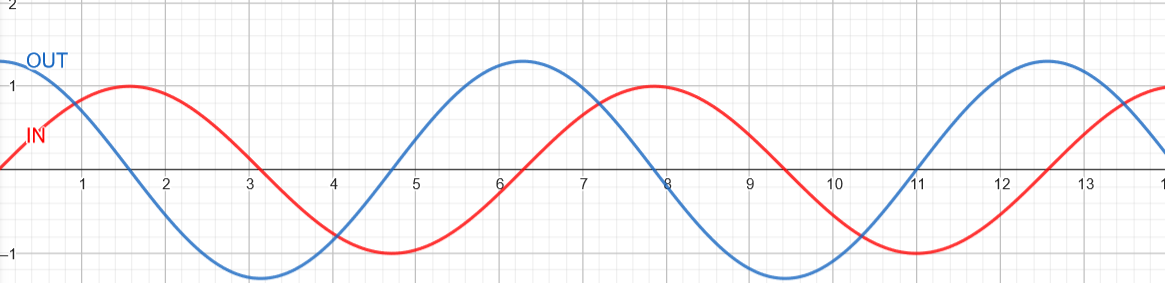
\includegraphics[width=0.8\linewidth]{immagini/integratore1} 	
   			\label{fig:integratore1}
   		\end{figure}  		
   		E se l'ingresso ha un'elevata frequenza? Sia ad esempio $IN = \sin(10x) \Rightarrow OUT = -0.6(-\cos(10x))$.
   		
   		Guardando il grafico del guadagno, questo per frequenze elevate fornisce valori minori, significa che in uscita il segnale avrà ampiezze minori, sarà più piccolo. 
   		\begin{figure}[H]
   			\centering
   			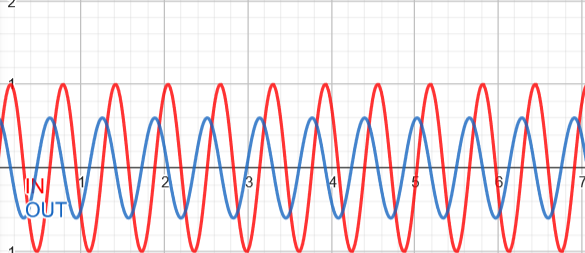
\includegraphics[width=0.7\linewidth]{immagini/integratore2}   	
   			\label{fig:integratore2}
   		\end{figure} 		
   		E per frequenze minori? Sia ad esempio $IN = \sin(0.3x) \Rightarrow OUT = sgn(-10(-\cos(0.3x)))$.
   		
   		Guardando il grafico del guadagno, si vede che per frequenze minori il segnale in uscita avrebbe ampiezza infinita, ma ricordando che al massimo si potrà avere la frequenza di alimentazione l'integratore va in saturazione e si ottiene in uscita un'onda quadra. 
   		\begin{figure}[H]
   			\centering
   			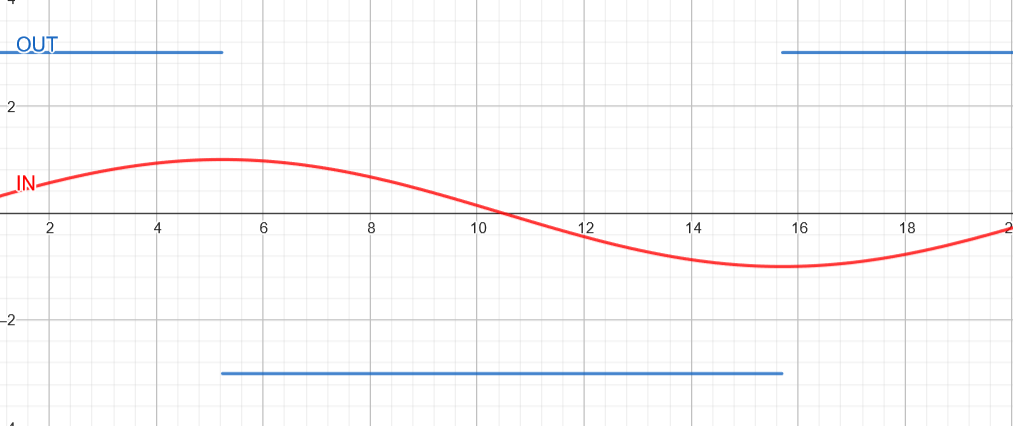
\includegraphics[width=0.7\linewidth]{immagini/integratore3}   	
   			\label{fig:integratore3}
   		\end{figure} 
\newpage   		 	
   	 	Per evitare la saturazione si aggiunge un resistore in parallelo al ramo di feedback.   	 	
   	 	\begin{figure}[H]
   	 		\centering
   	 		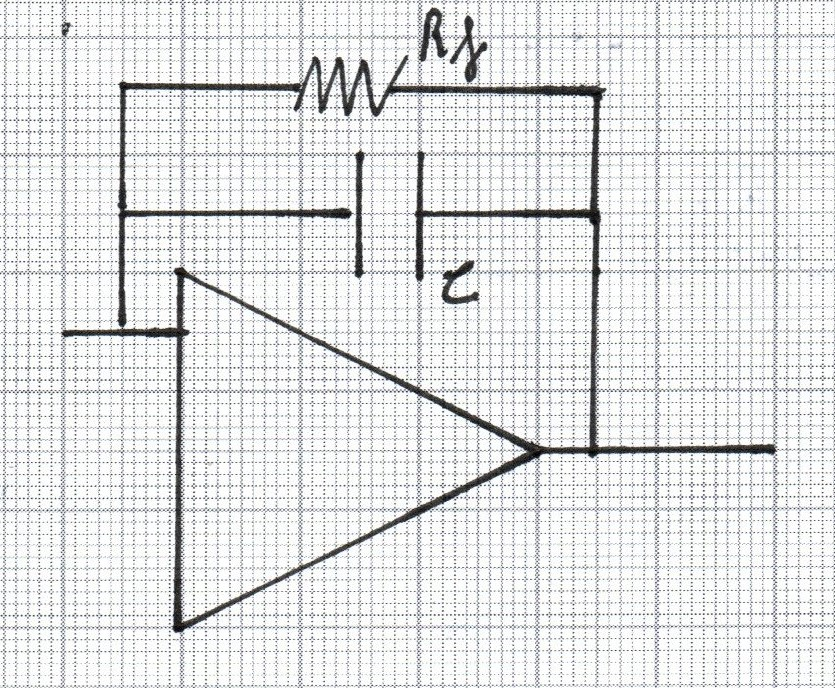
\includegraphics[width=0.3\linewidth]{immagini/mm(9)}
   	 		\label{fig:mm9}
   	 	\end{figure}   	 	
   	 	In questo modo:
   	 	\begin{eqnarray*}
   	 		V_{out} = - {Z_{\parallel}\over Z_{R_i}}V_i = -{Z_{R_f}Z_C\over(Z_{R_f}+Z_C)Z_{R_i}}V_i \\
   	 		V_{out} = -{R_f\over(j\omega R_fC+1)R_i}V_i
   	 	\end{eqnarray*}   	
    	Si proceda a razionalizzare per trovare il guadagno:   	
   		\[\begin{split}
   			V_{out} = -{R_f\over R_i}\dfrac{1-j\omega R_fC}{1+(\omega R_fC)^2)V_i} \Rightarrow G = {R_f\over R_i} \dfrac{1}{1+(\omega R_fC)^2}\sqrt{1+(\omega R_fC)^2} \Rightarrow \\ G = {R_f\over R_i} \dfrac{1}{\sqrt{1+(\omega R_fC)^2}}
   		\end{split}\]   		
   		\begin{figure}[H]
   			\centering
   			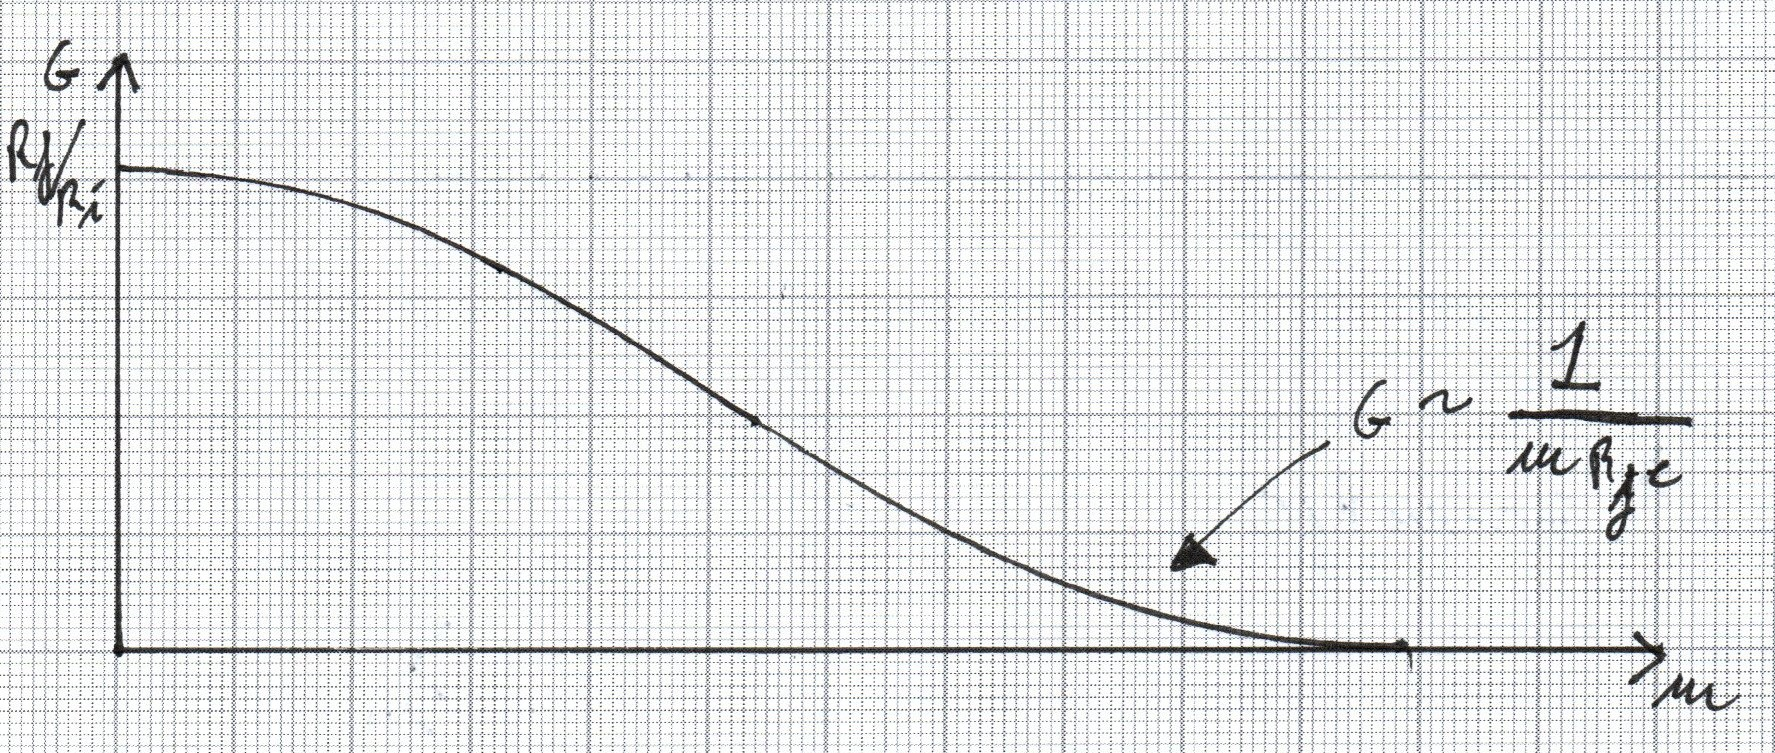
\includegraphics[width=0.5\linewidth]{immagini/mm(10)}
   			\label{fig:mm10}
   		\end{figure}   		    		
   		Per $\omega\rightarrow\infty ~~ G\approx{1\over\omega R_iC}$ per cui continua ad integrare. 
   		
   		Si ricordi poi da elettrotecnica che per $\omega\uparrow$ il condensatore si comporta come un circuito aperto, mentre per $\omega\downarrow$ il condensatore si comporta come un circuito chiuso, un corto circuito che fa passare tutto il segnale, saturando. 
   		
   		In questo caso l'integratore, non saturando, i comporta a basse frequenze come un classico amplificatore invertente. \newline 
   		
   		Ad esempio l'integratore potrà essere utilizzato per stabilire l'entità del segnale costante, infatti, per un andamento in ingresso dato da un'onda quadra, si sceglie di integrare un segnale esponenziale, in questo modo diminuendo la frequenza dell'onda quadra gli esponenziali vengono via via tagliati fino ad ottenere una linea, ovvero l'integrale del segnale costante desiderato, il segnale uscente diviene così a dente di sega. 
\end{adjustwidth}
\newpage
\subsection{Circuito Chiuso invertente derivatore}
\begin{adjustwidth}{2in}{}    		   		
   		\begin{figure}[H]
   			\centering
   			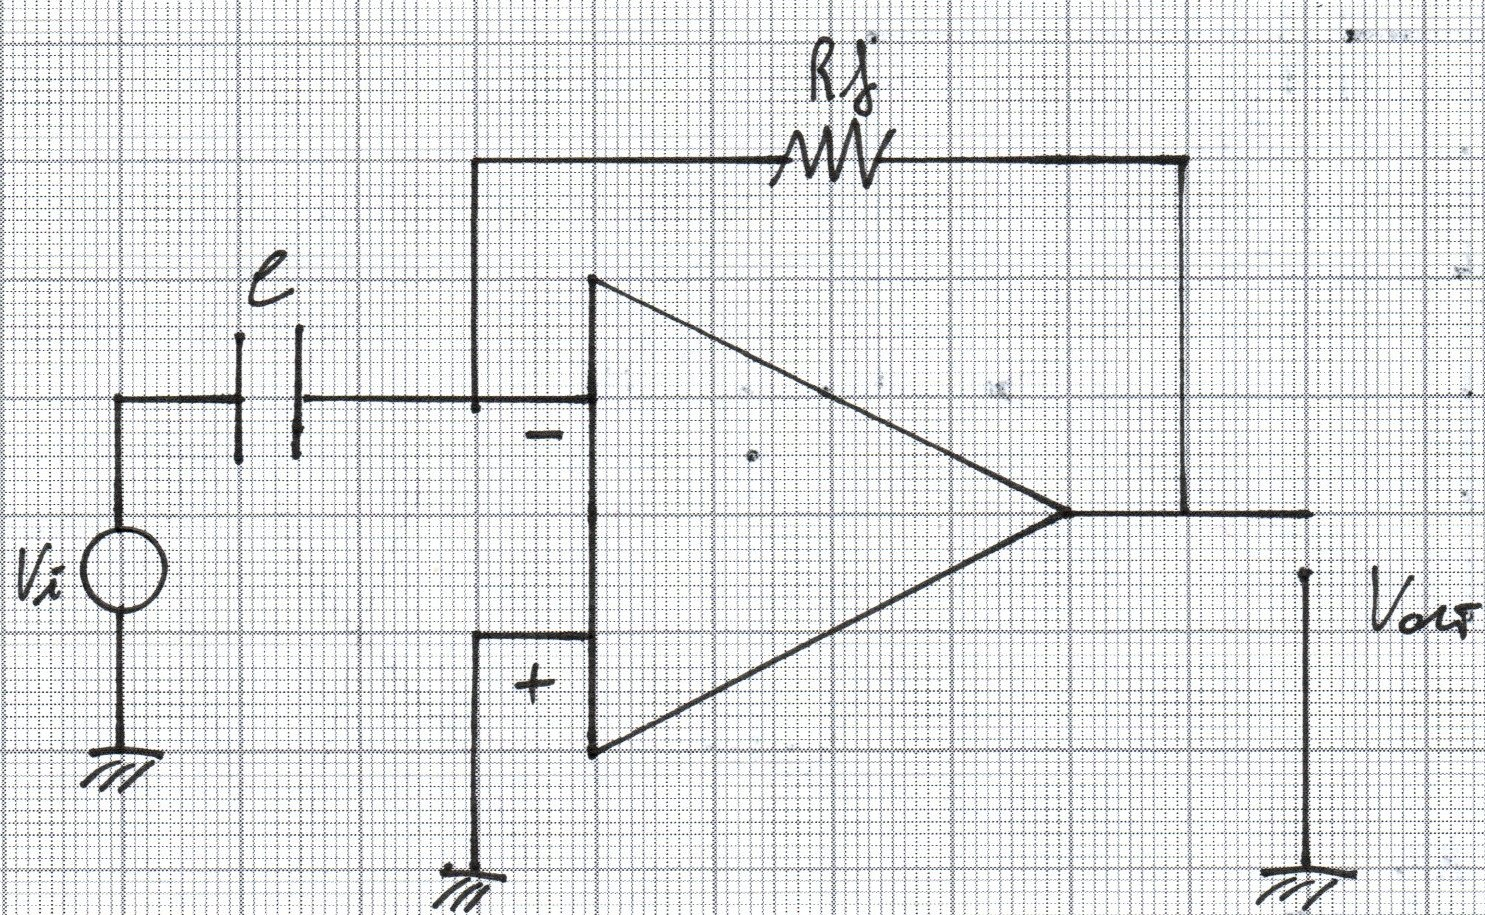
\includegraphics[width=0.5\linewidth]{immagini/mm(11)}
   			\label{fig:mm11}
   		\end{figure}   		  		
   		\[V_{out} = -{Z_{R_f}\over Z_C}V_i = -j\omega R_fCV_i\]
   		È questo segnale la derivata del segnale in ingresso? 
   		\begin{eqnarray*}
   			V_i = V_0e^{j\omega t}\Rightarrow{dV_i\over dt} = j\omega V_0e^{j\omega t} = j\omega V_i \Rightarrow V_i =  {dV_i\over dt}{{1\over j\omega}}\\
   			V_{out} = -j\omega R_fCV_i = -j\omega R_fC{dV_i\over dt}{{1\over j\omega}} = -R_fC{dV_i\over dt} \\
   			   		V_{out} = -R_fC{dV_i\over dt}
   		\end{eqnarray*}
   		Il Guadagno del circuito integratore è: 
   		\[G = \left|{V_{out}\over V_{i}}\right| = \omega R_fC\]  		
   		L'andamento è lineare tuttalpiù fino al valore di saturazione.   		
   		\begin{figure}[H]
   			\centering
   			\begin{tikzpicture}
   				\begin{axis}[
   					axis lines = left,
   					xlabel = \(\omega\),
   					ylabel = {\(G\)},
   					xticklabels=\empty,yticklabels=\empty]
   					\addplot [domain=0:10, 
   					samples=100, line width=1pt
   					] {
   						x
   					};
   				\end{axis}
   			\end{tikzpicture}
   		\end{figure}  
\newpage  		
   		Il segnale che si vedrà in uscita sarà derivato, invertito e amplificato. Sia ad esempio $IN = \sin(x) \Rightarrow OUT = -\cos(x)$.
   		\begin{figure}[H]
   			\centering
   			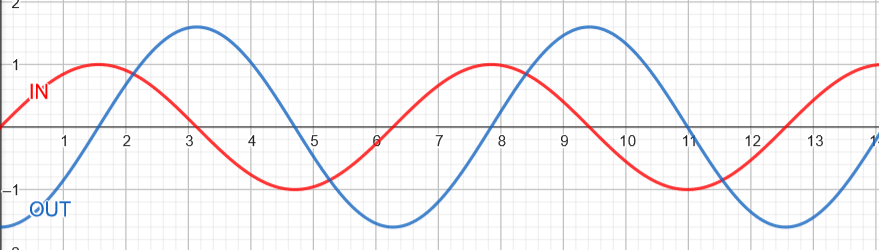
\includegraphics[width=0.7\linewidth]{immagini/integratore4}	
   			\label{fig:integratore4}
   		\end{figure}
   		In questo caso osservando il grafico del guadagno, aumentando la frequenza l'uscita sarà più amplificata. 
   		
   		Come si evita in questo caso la saturazione? Con una resistenza in serie al condensatore.   		
   		\begin{figure}[H]
   			\centering
   			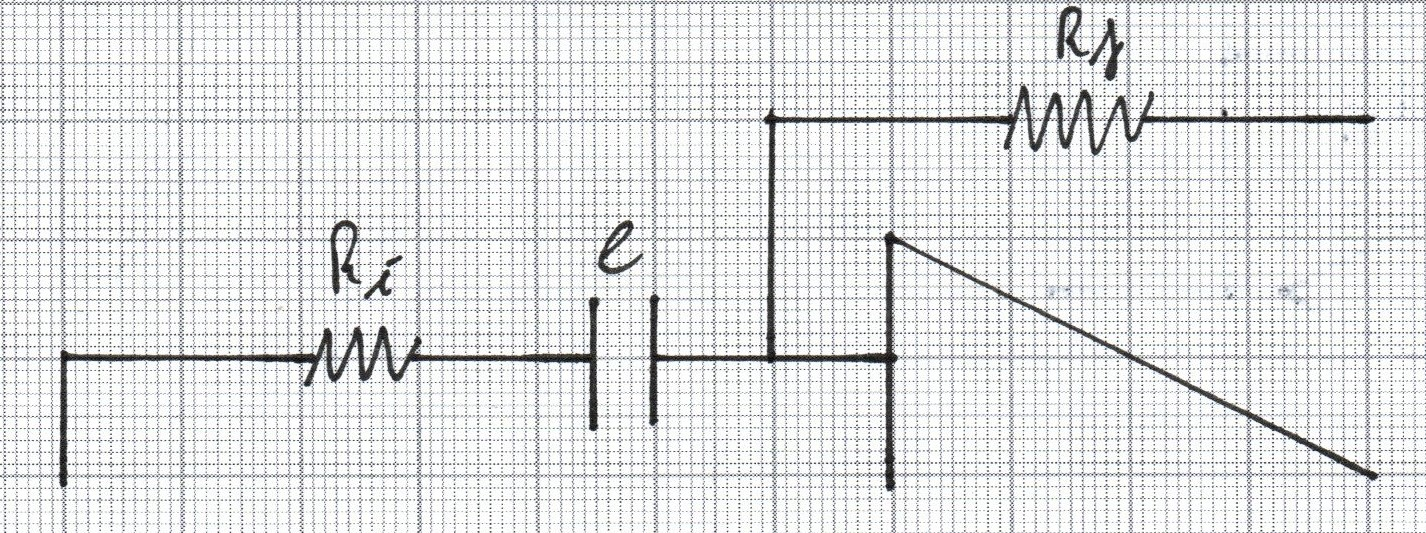
\includegraphics[width=0.5\linewidth]{immagini/mm(12)}
   			\label{fig:mm12}
   		\end{figure} 		
   		Per cui se $\omega\uparrow$ il condensatore si comporta come un cortocircuito. 
   		
   		\[V_{out} = -{Z_{R_f}\over Z_{R_i} + Z_C} = -\dfrac{R_f}{R_i + {1\over j\omega C}}V_i = -\dfrac{j\omega R_fC}{1+j\omega R_iC}V_i \] 
   		Razionalizzando ottengo:
   		\[V_{out} = - \dfrac{j\omega R_f C}{1+(\omega R_iC)^2}(1-j\omega R_iC)V_i = \dfrac{\omega R_fC}{1+(\omega R_iC)^2}\left[-j-\omega R_iC\right]V_i\]
   		Il guadagno sarà analogamente pari a: 
   		\[ G = \dfrac{\omega R_fC}{\sqrt{1+(\omega R_iC)^2}}\]
\begin{figure}[H]
	\centering
	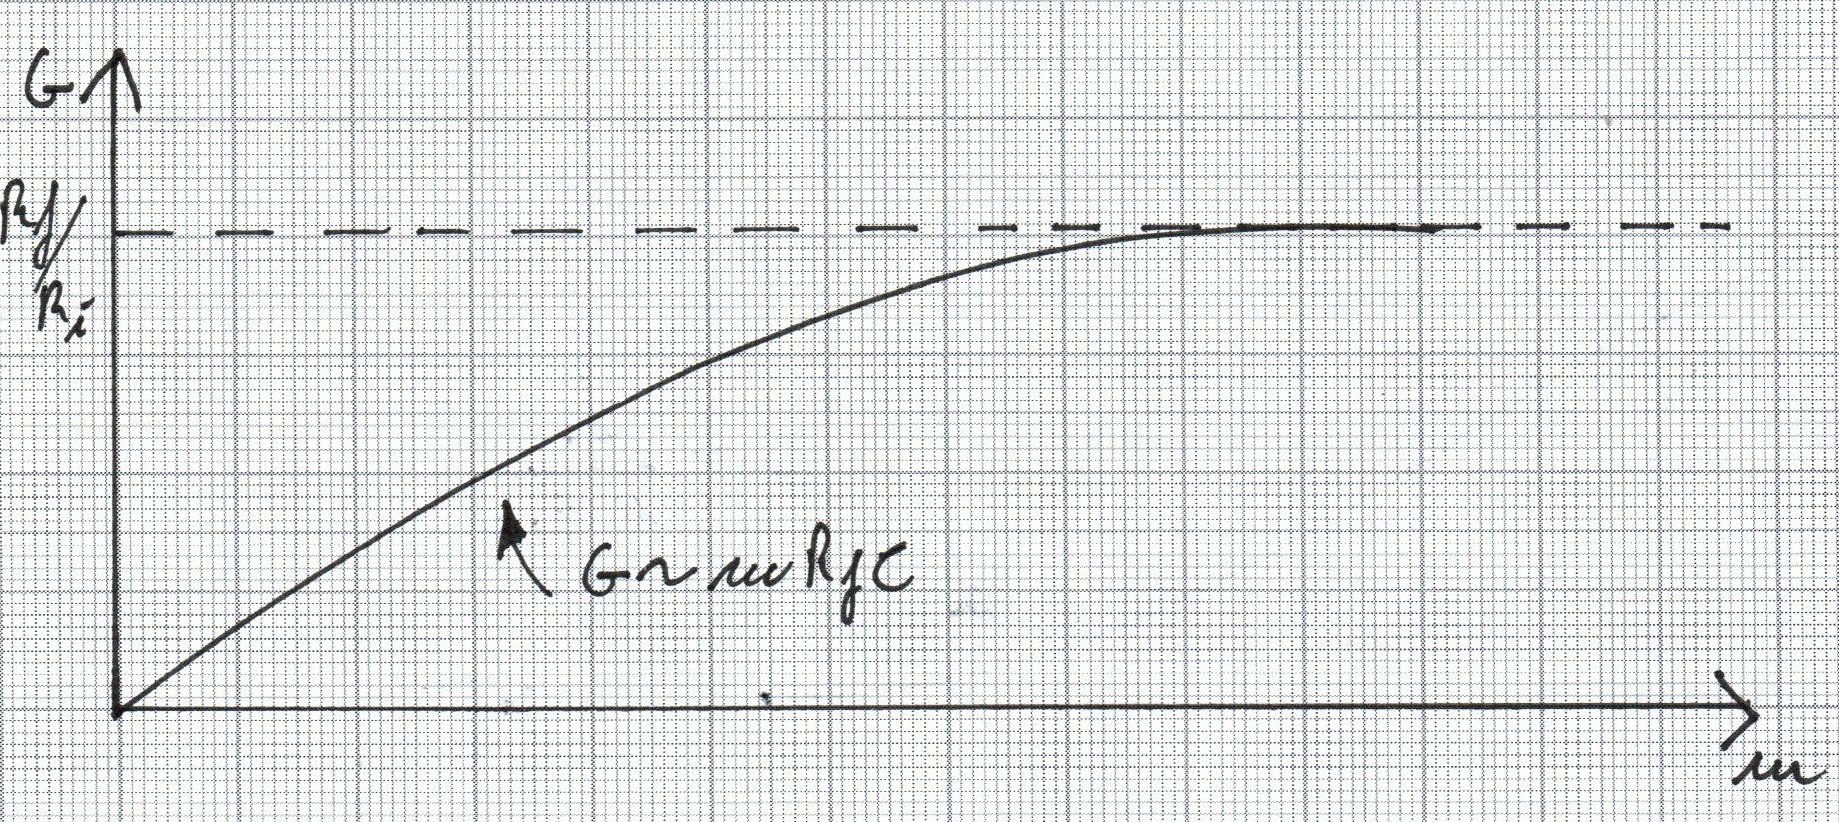
\includegraphics[width=0.5\linewidth]{immagini/mm(13)}
	\label{fig:mm13}
\end{figure}
   		Per cui per $\omega\rightarrow\infty ~~ G\rightarrow{R_f\over R_i}$ e per $\omega\downarrow ~~ G \approx\omega R_fC$. \newline 
\end{adjustwidth}
\newpage
\subsection{Circuiti Convertitori}
\subsubsection{Tensione-Corrente}
\begin{adjustwidth}{2in}{}      		
   		Questo tipo di circuito viene utilizzato quando si vuole avere una corrente in uscita corrispondente numericamente ad un valore di tensione di ingresso, a parte un fattore 1000, questo applicato alla corrente per non bruciare le resistenze. 
\begin{figure}[H]
	\centering
	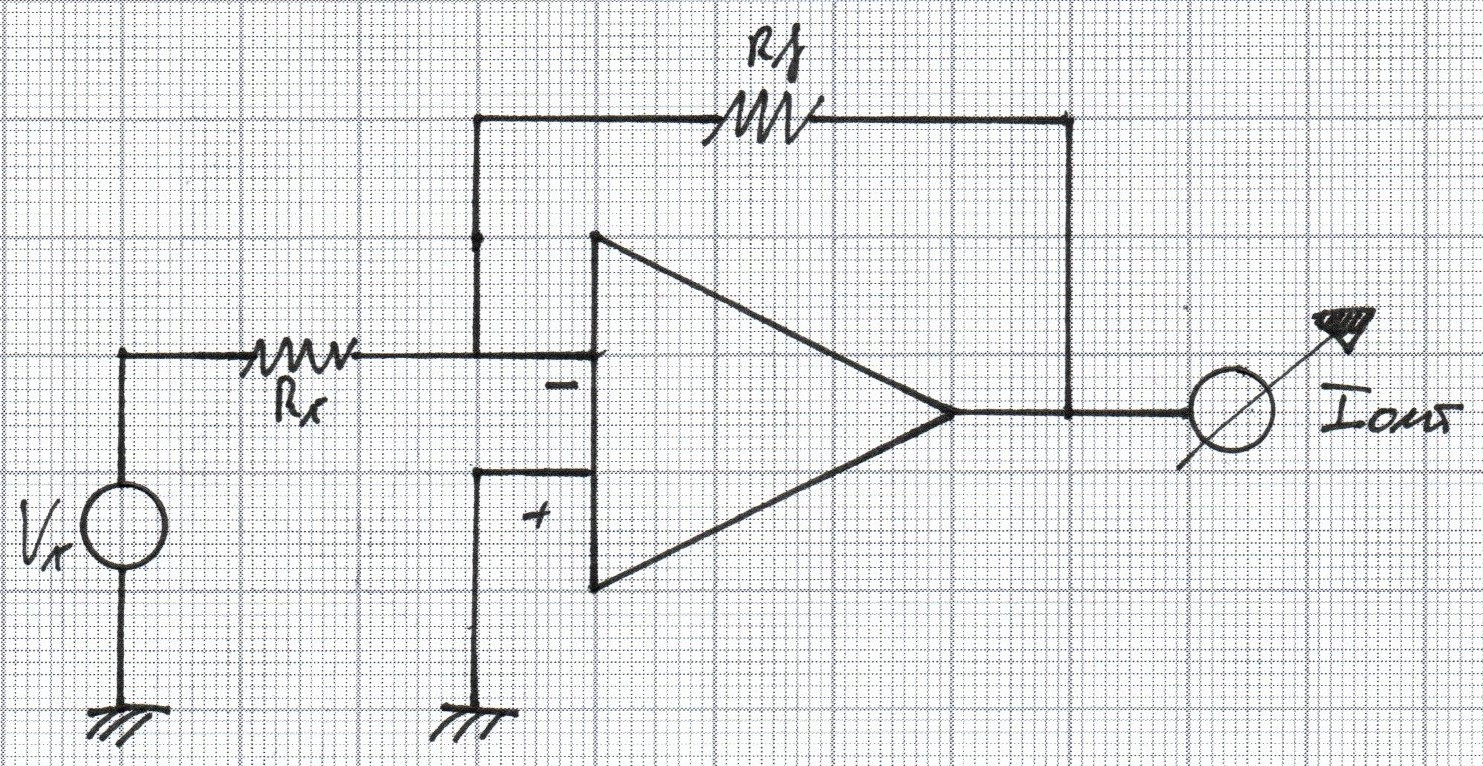
\includegraphics[width=0.5\linewidth]{immagini/mm(14)}
	\label{fig:mm14}
\end{figure}
   		\[I_{out} = {V_i\over R_i}\]   		
   		Ad esempio se si vuole misurare una corrente a partire da un ingresso di $5 V$ si sceglierà una $R_i = 1k\Omega$ per ottenere una corrente in uscita pari a $I_{out} = 5 mA$.  
\end{adjustwidth}
%\newpage
\subsubsection{Corrente-Tensione}
\begin{adjustwidth}{2in}{} 
   		Equivalente si avrà, se in uscita si vuole misurare una tensione a partire da un ingresso in corrente.    		
   		\begin{figure}[H]
   			\centering
   			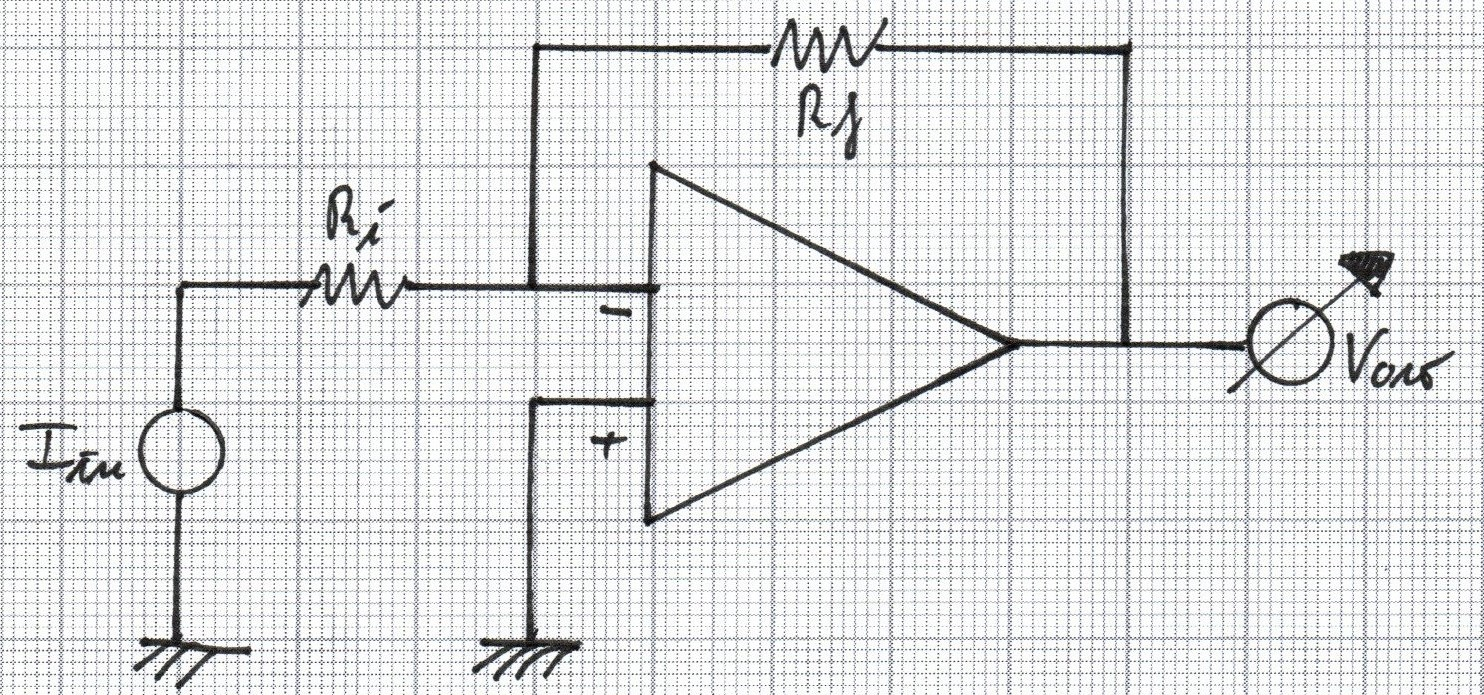
\includegraphics[width=0.5\linewidth]{immagini/mm(15)}
   			\label{fig:mm15}
   		\end{figure}   		
   		\[I_{in} = -{V_{out}\over R_f} \Rightarrow V_{out} = -R_fI_{in}\]   		
   		Ad esempio se si vuole misurare una tensione a partire da un ingresso di $3 mA$ si sceglierà una $R_f = 1k\Omega$ per ottenere una tensione in uscita pari a $V_{out} = 3 V$.  
\end{adjustwidth}
\newpage
\section{Circuito Chiuso non Invertente}
\begin{adjustwidth}{2in}{}   		
   		Usato per ottenere in uscita un segnale dello stesso segno di quello in entrata. 
\begin{figure}[H]
	\centering
	\scalebox{1.5}{\begin{circuitikz}
			%\draw [help lines] (0,0) grid (10,10);			
			\draw (5,1) node[op amp, anchor=+] (OA1) {};    % Amplificatore
			\draw (OA1.+) to[european voltage source, l_=$V_i$] (5,-0.5) node[ground]{};       % Ramo non invertente a terra
			\draw (OA1.-) to [R, l_=$R_i$] (3,2) to [short] (3,-0.5) node[ground]{}; % Ramo invertente col segnale
			\draw (OA1.-) -- (5,3) to [R, l=$R_f$] (5,3 -| OA1.out) -- (OA1.out); % Ramo di feedback
			\draw (7.5,1) -- (7.5,-0.5) node[ground]{$V_{out}$};	% Uscita		
	\end{circuitikz}}
\end{figure}
   		L'ipotesi di partenza è quella per cui si considera sempre valido il principio di massa virtuale:
   		\[V_+ = V_i = V_-\]
   		Ottenendo:
   		\[{0-V_i\over R_i} = {V_i-V_{out}\over R_f} \Rightarrow V_{out} = V_i\left(1 + {R_f\over R_i}\right)\]
   		Come volevasi dimostrare, si ottiene un segnale dello stesso segno di quello in ingresso. \newline 
   		
   		Il guadagno è pari a:
   		\[G = 1 + {R_f\over R_i}\]
   		Sempre positivo.
   		
   		Per cui se con la configurazione invertente si può anche deamplificare il segnale, in questo caso, non si può, perché anche se $ R_f=R_i=0$ il guadagno è sempre unitario, che ottiene o per $R_i\uparrow$ o per $R_f\uparrow0$. \newline 
\end{adjustwidth}
%\newpage
\subsection{Circuito Buffer o Disaccoppiatore}
\begin{adjustwidth}{2in}{}     		
   		Configurazione non invertente in cui $R_f = 0\Rightarrow V_{out} = V_i$ usato per minimizzare l'errore di inserzione, per evitare che la fonte del segnale sia influenzata da qualsiasi corrente o tensione.   		
   		\begin{figure}[H]
   			\centering
   			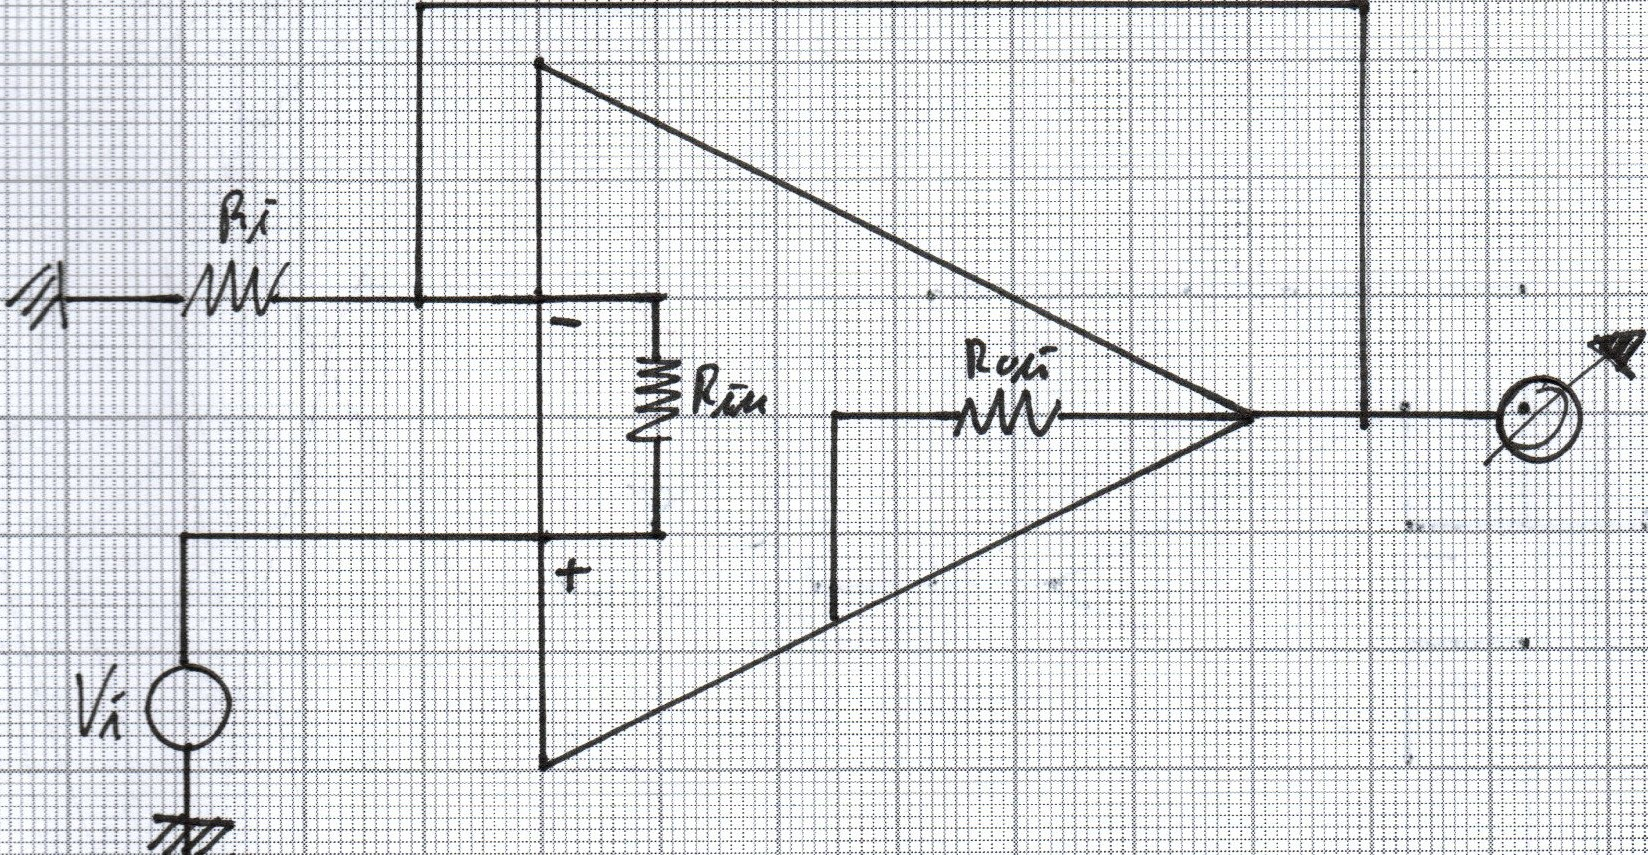
\includegraphics[width=0.5\linewidth]{immagini/mm(16)}
   			\label{fig:mm16}
   		\end{figure}  		
   		Con un attacco diretto al multimetro di avrebbe:
   		\[\varepsilon_{ins} = \dfrac{R_{batteria}}{R_{multimetro}}\]
   		Interponendo un circuito buffer si avrebbe: 
   		\[\varepsilon_1 = {R_b\over R_{in}}\rightarrow0\hspace{1cm} \varepsilon_2 = {R_{out}\over R_{m}}\rightarrow0\]
   		
   		In questo caso, con la misura di tensione di una batteria si vuole minimizzare l'errore di inserzione nella misura data da una $R_b\uparrow$ su cui scorre corrente per cui si potrebbe misurare un valore falsato, minore.  
\end{adjustwidth}
%\newpage
\subsection{Circuito Sommatore Non Invertente}
\begin{adjustwidth}{2in}{}    		
   		Come per la configurazione invertente, si vuole ottenere \[V_{out} = \sum V_i = V_1 + V_2 + V_3\]   		
   		\begin{figure}[H]
   			\centering
   			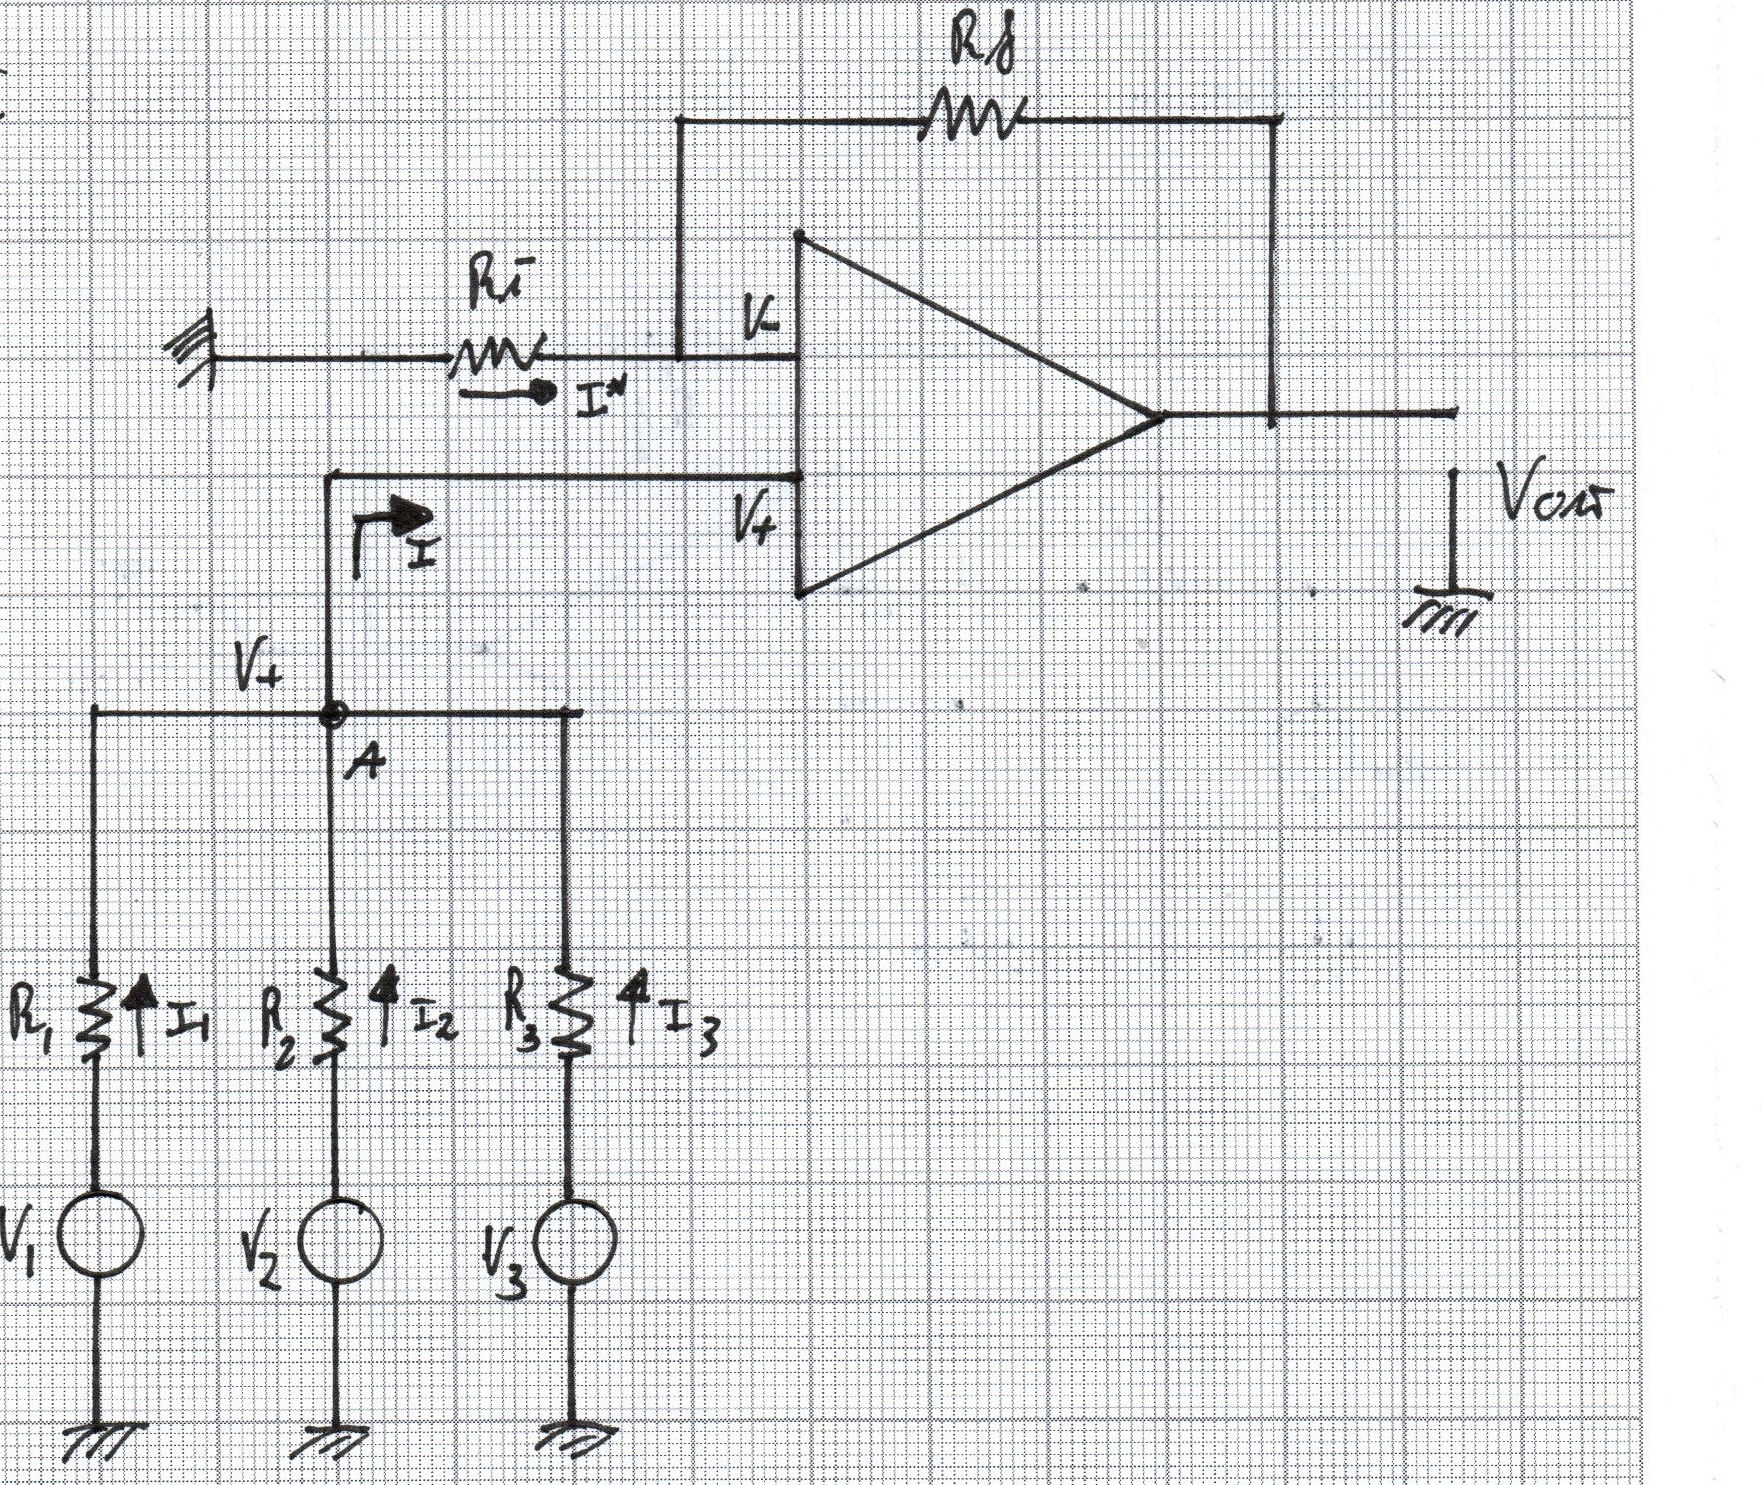
\includegraphics[width=0.5\linewidth]{immagini/mm(17)}
   			\label{fig:mm17}
   		\end{figure}   		
   		\[I* = {-V_+\over R_i} = {V_+-V_{out}\over R_i} \Rightarrow V_{out} = \left(1 + {R_f\over R_i}\right)V_+\]
   		Sul nodo A:   		
   			\[I_1 + I_2 + I_3 = I\]    			
   			\[{V_1-V_+\over R_1} + {V_2-V_+\over R_2} + {V_3 - V_+\over R_3} = 0\]   		
   		Scegliendo $R_1 = R_2 = R_3 = R$ si ottiene: 
   		\[V_+ = {V_1+V_2+V_3\over3}\]
   		
   		Per cui:
   		\[V_{out} = \left(1 + {R_f\over R_i}\right){V_1+V_2+V_3\over3} \] 
   		Per avere un sommatore vasta scegliere $R_f = 2R_i$, per avere invece un circuito mediatore, si sceglie $R_f = 0$, si realizza un buffer cortocircuitando il ramo di feedback.  
\end{adjustwidth}
\newpage
\subsection{Circuito Sottrattore Non Invertente}
\begin{adjustwidth}{2in}{}   
   		Dati due segnali in ingresso, in uscita se ne vuole misurare la differenza: $V_{out} = V_2 - V_1$.    		
\begin{figure}[H]
	\centering
	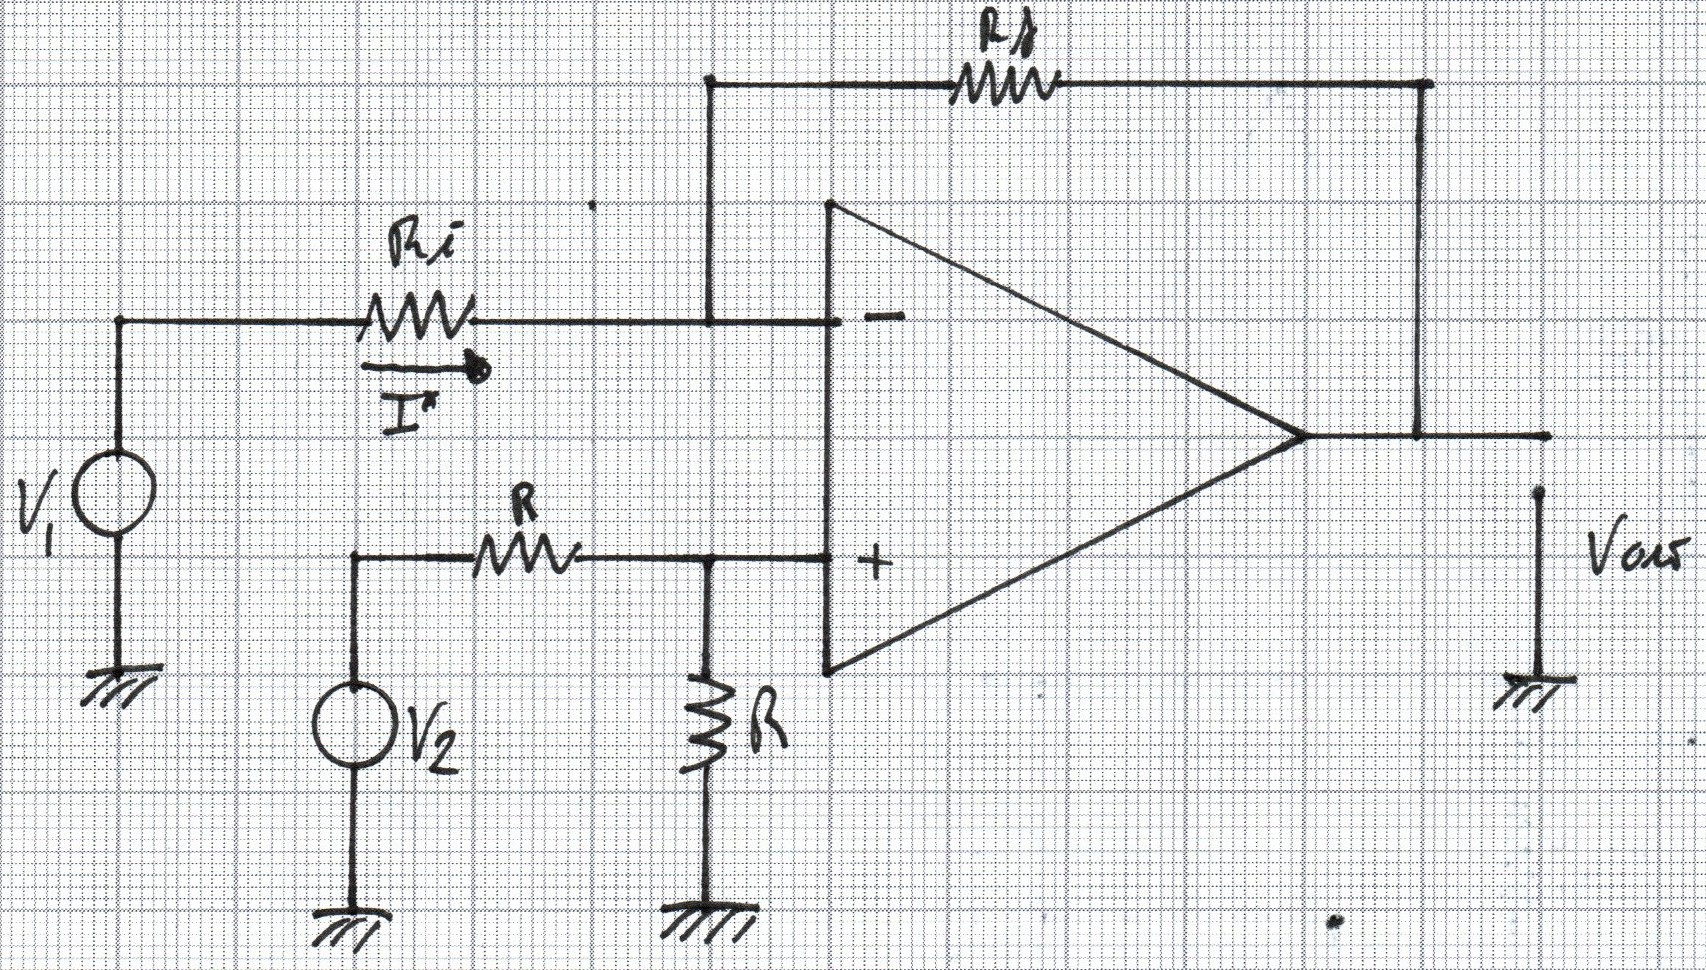
\includegraphics[width=0.5\linewidth]{immagini/mm(18)}
	\label{fig:mm18}
\end{figure}   		
   		La resistenza aggiuntiva a massa ha la funzione di partitore di tensione:
   		\[V_2 = I2R; V_+ = IR \Rightarrow V_+ = {1\over2}V_2\]
   		Applicando la classica formula dell'amplificatore ottengono:
   		\[I* = {V_1-V_+\over R_i}= = {V_+-V_{out}\over R_f}\Rightarrow{R_f\over R_i}V_1 - {R_f\over R_i}V_+ = V_+ - V_{out} \]
   		\[V_{out} = \left(1+{R_f\over R_i}\right)V_+ - {R_f\over R_i}V_1 = \left(1+{R_f\over R_i}\right){V_2\over2}- {R_f\over R_i}V_1 \]
   		Prendendo $R_f = R_i$ si ottiene:
   		\[V_{out} = V_2 - V_1\]
\end{adjustwidth}
%\newpage
\subsection{Amplificatore per Strumentazione}
\begin{adjustwidth}{2in}{} 		
   		È usato per amplificare la differenza tra due segnali in ingresso con un guadagno variabile $G\nearrow$:
   		\[V_{out} = G\nearrow(V_2-V_1)\] 
   		Cosa deve fare un amplificatore per strumentazione?
   		\begin{enumerate}
   			\item Disaccoppiare i segnali in ingresso $\rightarrow$ Buffer
   			\item Sottrarre i segnali in ingresso $\rightarrow$ Sottrattore
   			\item Moltiplicare il segnale in uscita per un guadagno variabile $\Rightarrow$ L'amplificazione de segnale dev'essere variabile. 
   		\end{enumerate}  	
\begin{figure}[H]
	\centering
	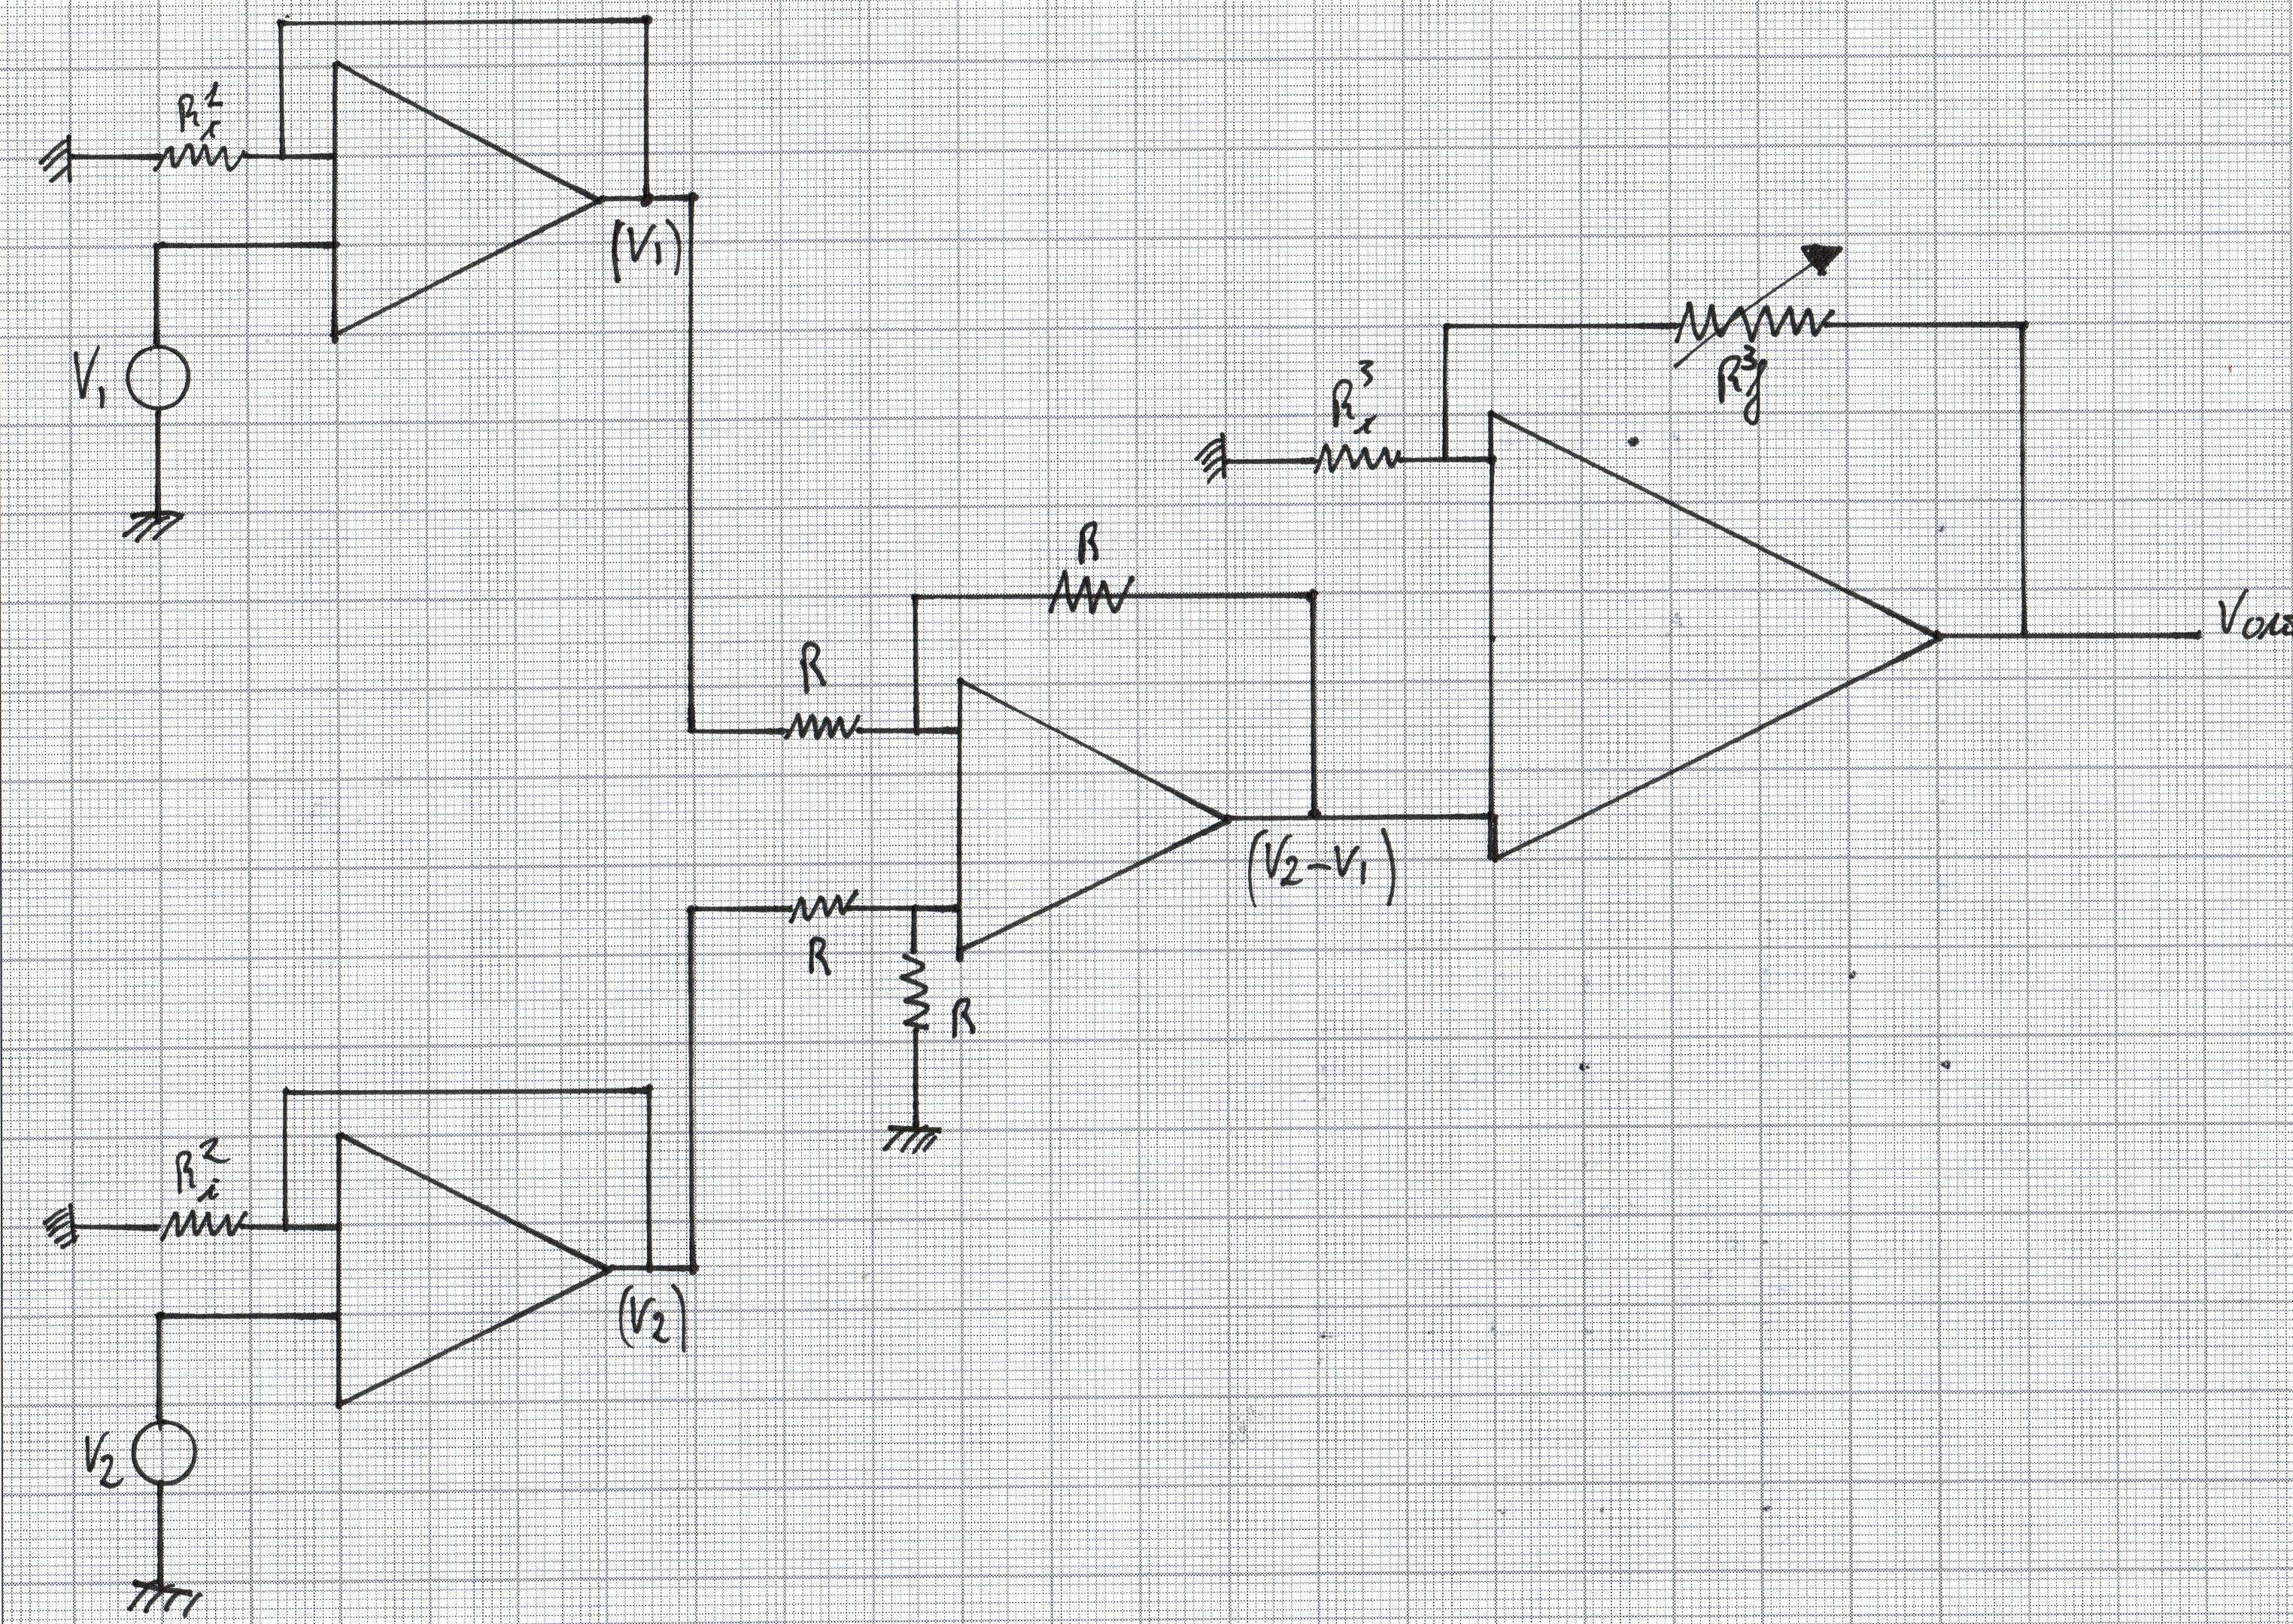
\includegraphics[width=0.5\linewidth]{immagini/mm(19)}
	\label{fig:mm19}
\end{figure}  		
   		In questo modo
   		\[V_{out} = \left(1 + {R_{f3}\nearrow\over R_i3}\right)(V_2-V_1)\]
   		In cui $ R_{f3}\nearrow $ non è nient'altro che un potenziometro. \newline

   		Ad esempio se $R_{i3} = 10 ~ k\Omega; R_{f3}\nearrow = (0\div10) ~ k\Omega$ si avrà quando $C\equiv A$
   		\[V_{out} = V_2 - V_1\] E quando $C\equiv\max$  \[V_{out} = \left(1 + {10 k\Omega\over 10 k\Omega}\right)(V_2-V_1) = 11(V_2-V_1)\]
\end{adjustwidth}
%\newpage
\section{Amplificatori Reali}
\begin{adjustwidth}{2in}{}
   		Si sono trattati finora solo amplificatori ideali in cui:
   		\[V_{out} = A(V_+V_-)\]
   		Dall'esperienza si nota che se si cortocircuitano morsetto positivo e morsetto negati dell'amplificatore, si misura una $\Delta V\ne 0$ in contrasto con la teoria, che considerata la costante $A$ essere molto alta, porta immediatamente a saturazione il segnale in ingresso. \newline 
   		
   		Nella realtà l'equazione dell'amplificatore reale è:
   		\[V_{out} = A_+V_+ - A_-V_-\]
   		Per cui ho guadagni differenti per i differenti morsetti, ci si riconduce facilmente al caso ideale non appena \(A_+=A_-\). \newline 
   		
   		Si definiscono \textbf{Tensione Differenziale} e \textbf{Tensione di Modo Comune} rispettivamente le seguenti quantità:
   		\[V_d = V_+-V_- \hspace{1cm} V_{cm} = {V_++V_-\over2}\]
   		In questo modo: 
   		\[\begin{cases}
   			V_- = V_+ - V_d \\
   			V_{cm} = {V_+ + V_+ - V_d\over2} = V_+ - {V_d\over2}
   		\end{cases} \hspace{1cm} \begin{cases}
   		V_+ = V_{cm} + {V_d\over2} \\
   		V_- = V_{cm} - {V_d\over2}
   		\end{cases}\]
   		Così facendo:
   		\begin{eqnarray*}
   			V_{out} = A_+V_{cm} + A_+{V_d\over2} - A_-V_{cm} + A_-{V_d\over2} \\
   			V_{out} = \underbrace{ \left(A_+-A_-\over2\right)}_{A_d}V_d + \underbrace{\left(A_+-A_-\right)}_{A_{cm}}V_{cm}
   		\end{eqnarray*}
   		In cui si identifica il guadano differenziale $A_d$ e il guadagno di modo comune $A_{cm}$ quello che determina l'errore rispetto all'idealità, per cui se $A_+=A_-$ è nullo e riconduce all'idealità. \newline 
   		
   		\[V_{out} = A_dV_d + A_{cm}V_{cm}\]
   		Con rigorosamente $A{cm}<A_d$. 
   		
   		Si indica poi con CMRR il rapporto di reiezione di modo comune ed indica la capacità di rigettare il guadagno di modo comune per avvicinarsi all'idealità, non considerando $V_{cm}$. 
   		\[CMRR = 20\log\left(A_d/A_{cm}\right)\] 
   		Più altro questo fattore è e migliore sarà l'amplificatore. 
\end{adjustwidth}
%\newpage
\subsubsection{Esercizio d'esame}
\begin{adjustwidth}{2in}{}
   		Disegnare il circuito elettrico che note tre tensioni in ingresso in uscita generi \({1\over RC}\int {V_1 + V_2 + V-3\over3}dt\). \newline 
   		
   		Si propende per un mediatore invertitore più un integratore invertitore.    		
   		\begin{figure}[H]
   			\centering
   			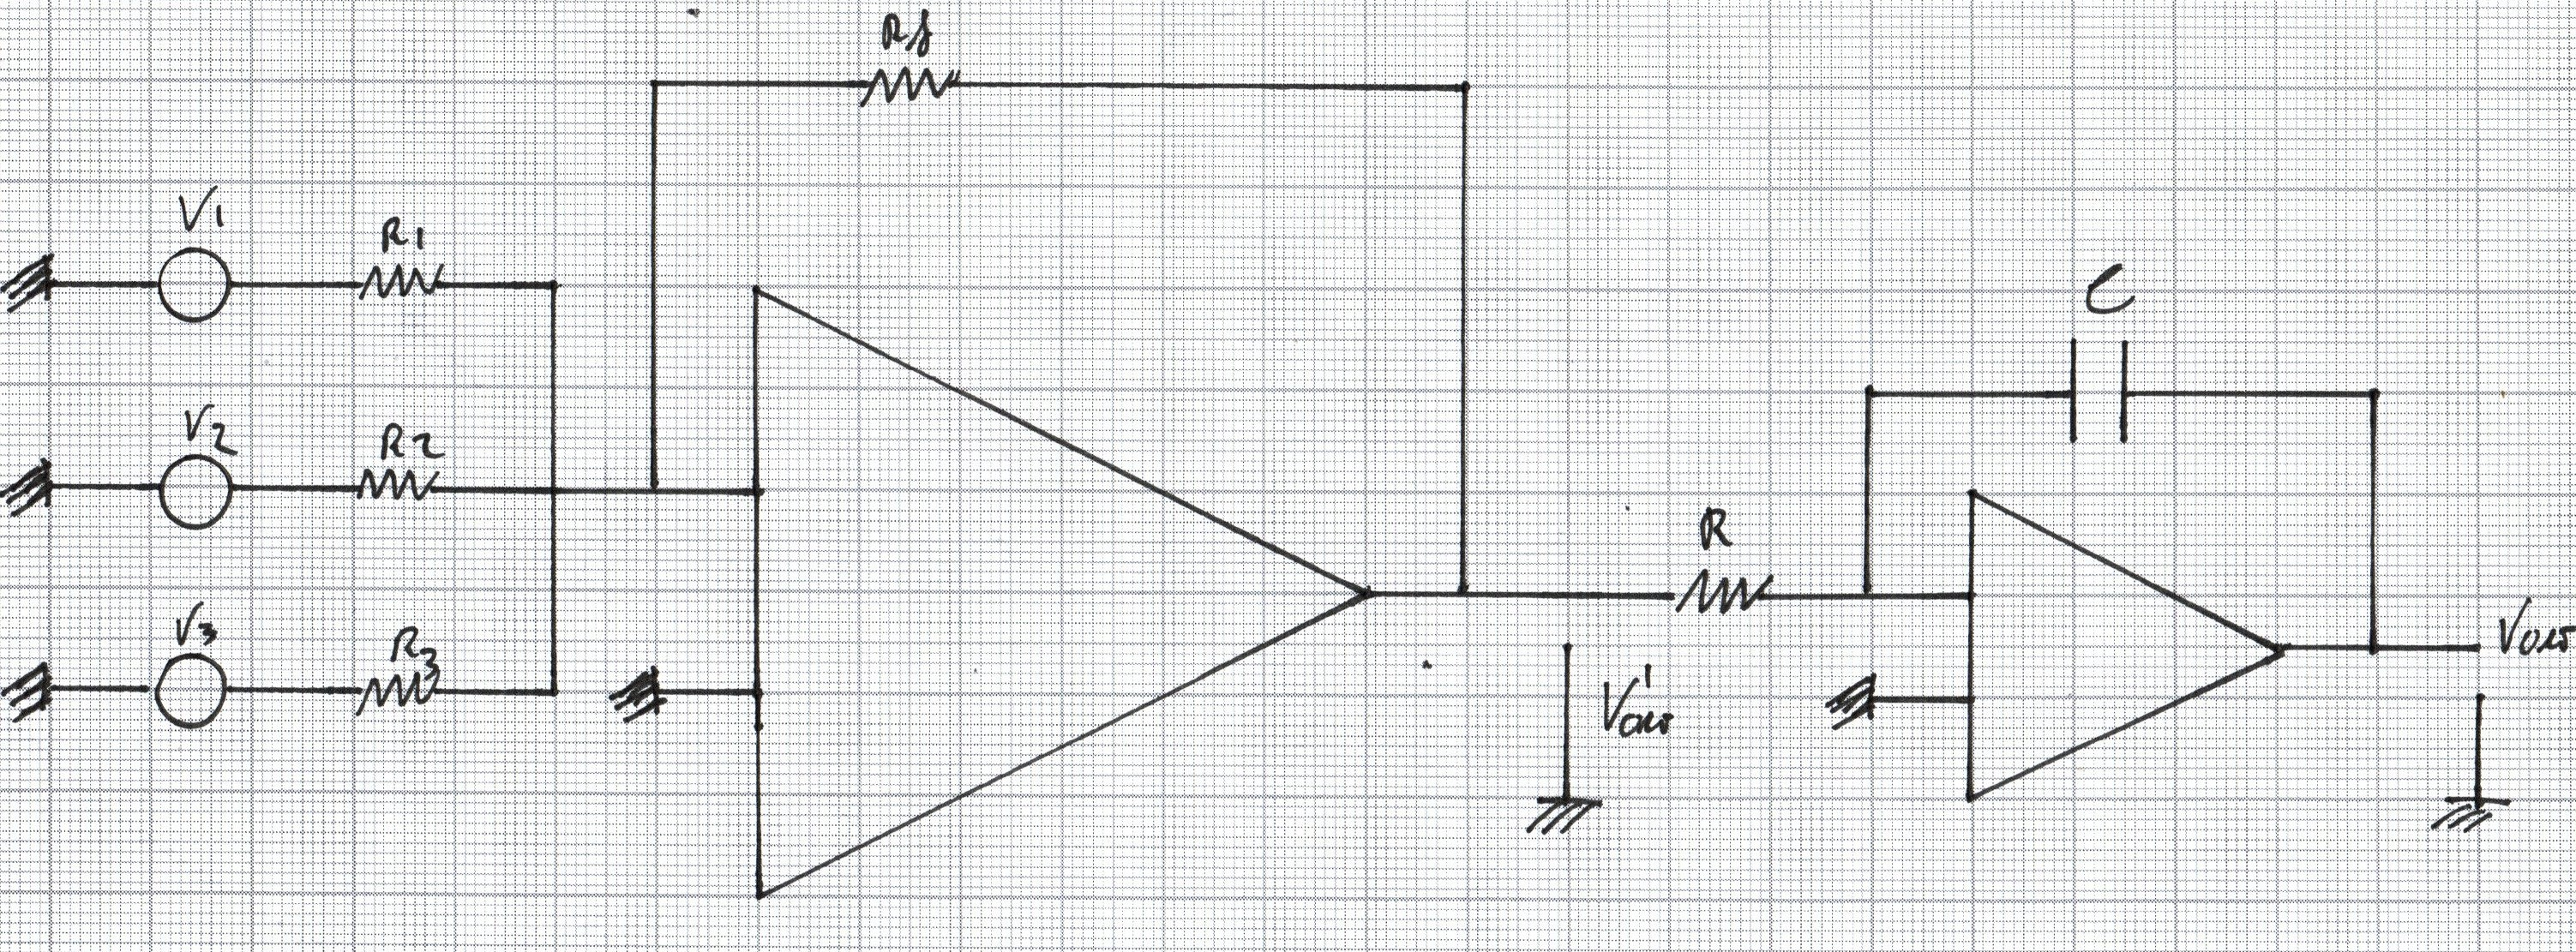
\includegraphics[width=0.5\linewidth]{immagini/mm(20)}
   			\label{fig:mm20}
   		\end{figure}   	
   		In questo modo:
   		\[{V_1\over R_1} + {V_2\over R_2} + {V_3\over R_3} = -{V'_{out}\over R_f} \Rightarrow -R_f\left({V_1\over R_1} + {V_2\over R_2} + {V_3\over R_3} \right)\]
   		Si scelgono $R_1=R_2=R_3 = 3R_f$, in modo da avere in output:
   		\[ V_{out} = -{1\over RC}\int -{V_1 + V_2 + V-3\over3}dt \]
\end{adjustwidth}
\newpage
\section{Filtri Attivi}
\begin{adjustwidth}{2in}{}
   		I filtri attivi sono filtri che oltre a filtrare il segnale lo amplificano, a differenza dei filtri passivi. Questi sono:
   		\begin{itemize}
   			\item Passa Basso 
   			\item Passa Alto
   			\item Passa Banda
   			\item A Reiezione di Banda o Filtro Notch. 
   		\end{itemize}
   		Sia un segnale scomposto Attraverso Fourier tramite una somma di soli seni: \(\sum_{i}^{n}A_i\sin(2\pi f_it)\), tale segnale può così essere scomposto in spettri di frequenze.
\begin{figure}[H]
	\centering
	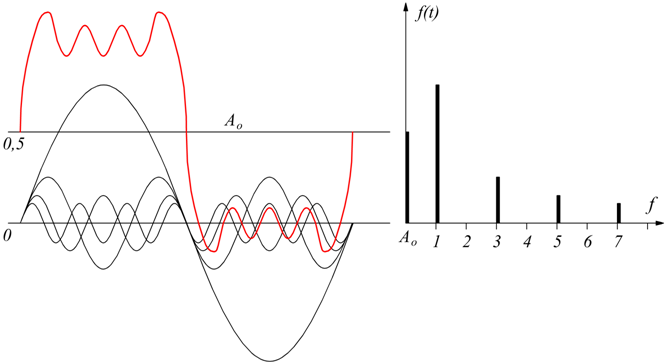
\includegraphics[width=0.5\linewidth]{immagini/16}
	\label{fig:16}
\end{figure}
\end{adjustwidth}
%\newpage
\subsection{Filtri Attivo Passa Basso}
\begin{adjustwidth}{2in}{}
   		Il filtro Passa Basso, imponendo una determinata frequenza di taglio $f_t$ permette il filtraggio delle alte frequenze. Il filtro ideale moltiplica per una costante che si indica come unitaria per semplicità (si ricordi che amplifica) gli spettri dei segnali che vuole far passare, si vuole così eliminare il segnale alle alte frequenze. 
\begin{figure}[H]
	\centering
	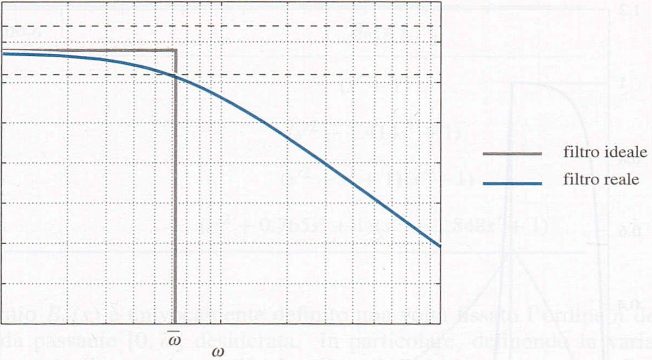
\includegraphics[width=0.5\linewidth]{immagini/screenshot002}
	\label{fig:screenshot002}
\end{figure}
   		Nel filtro reale la frequenza di taglio $f_t$ si trova dove è presente il 30\% di deamplificazione del segnale. 
   		
   		NB: è importante non moltiplicare il segnale per valori prossimi o uguali alla frequenza di taglio, perché il segnale verrebbe deamplificato. \newline 
   		
   		L'ordine del filtro indica la pendenza del guadagno, quanto è ovvero più vinci all'unita senza subire deamplificazione, da 1 a 4. 
   		\begin{figure}[H]
   			\centering
   			\scalebox{1.5}{\begin{circuitikz}
   					%\draw [help lines] (0,0) grid (10,10);			
   					\draw (5,1) node[op amp, anchor=+] (OA1) {};    % Amplificatore
   					\draw (OA1.+) to [C, l^=$C$] (5,-0.5) node[ground]{};       % Ramo non invertente 1 a terra
   					\draw (OA1.+) to [R, l^=$R$] (3,1) to[european voltage source, l_=$V_i$] (3,-0.5) -- (3,-0.5) node[ground]{}; % Ramo non invertente 2 col segnale
   					\draw (OA1.-) to [R, l_=$R_i$] (2,2) -- (2,-0.5) node[ground]{}; % Ramo invertente a terra
   					\draw (OA1.-) -- (5,3) to [R, l^=$R_f$] (5,3 -| OA1.out) -- (OA1.out); % Ramo di feedback
   					\draw (7.5,1) -- (7.5,-0.5) node[ground]{$V_{out}$};	% Uscita		
   			\end{circuitikz}}
   		\end{figure}
   	   		
   		\begin{figure}[H]
   			\centering
   			\scalebox{0.8}{\begin{circuitikz}
   					%\draw [help lines] (0,0) grid (5,5);			
   					\draw (0,0) to[european voltage source, l^=$V_i$] (0,5) -- (3,5) to [generic, l^=$Z_R$] (3,2.5) to [generic, l^=$Z_C$] (3,1) -- (3,0) -- (0,0); % Circuito 
   					\draw (3,2.5) 	to [short, -*]	(5,2.5); 
   					\draw (3,0.5) 	to [short, -*]	(5,0.5); 
   					\draw (5,0.5)to[open,v_>=$V_+$,*-*](5,2.5);
   			\end{circuitikz}}
   		\end{figure}
   		
   		Dal partitore si ottiene: 
   		\[\begin{cases}
   			V_i = I(Z_R + Z_C) \\
   			V_+ = IZ_C
   		\end{cases} \Rightarrow V_+ = \dfrac{Z_C}{Z_R+Z_C}V_i \Rightarrow V_+ =\dfrac{1}{1+j\omega RC}V_i\]
   		Noto $V_+$ si calcola $V_out$:
   		\[-{V_+\over R_i} = {V_+-V_{out}\over R_f}\Rightarrow V_{out} = \left(1+{R_f\over R_i}\right)V_+ = \left(1+{R_f\over R_i}\right)\dfrac{1}{1+j\omega RC}V_i\]
   		Razionalizzando:
   		\[ V_{out} = \left(1+{R_f\over R_i}\right)\dfrac{1-j\omega RC}{1+(\omega RC)^2}V_i \]
   		Allora il guadagno sarà:
   		\[G = \left(1+{R_f\over R_i}\right) \dfrac{1}{\sqrt{1+(\omega RC)^2}}\]
   	\newpage
   		Per $\omega\rightarrow0 ~~ G\rightarrow 1+{R_f\over R_i}$, per $\omega\rightarrow\infty ~~ G\rightarrow0$.    		
   		\begin{figure}[H]
   			\centering
   			\begin{tikzpicture}
   				\begin{axis}[
   					axis lines = left,
   					xlabel = \(\omega\),
   					ylabel = {\(G\)}, ymax=1.1,
   					xticklabels=\empty,yticklabels=\empty, extra y ticks={1}, extra y tick labels={$1+{R_f \over R_i}$}]
   					\addplot [domain=0:5, 
   					samples=100, line width=1pt
   					] {
   						1/((1+x^2)^(1/2))
   					};
   				\end{axis}
   			\end{tikzpicture}
   		\end{figure}   		
   		Dove c'è deamplificazione del segnale pari a 3 dB? Dov'è la frequenza di taglio? 
   		\[-3 dB = 20\log\left(G_{f_t}\over G_0\right) \Rightarrow -3 dB = 20\log\left(\dfrac{1}{\sqrt{1+(\omega RC)^2}}\right)\]
   		Ovvero ci si chiede quando: 
   		\[\dfrac{1}{\sqrt{1+(\omega RC)^2}} = {1\over\sqrt{2}} \Leftrightarrow \omega RC = 1 \Leftrightarrow \omega_{f_t} = 2\pi f_t = {1\over RC}\]
   		Infine:
   		\[f_t = {1\over 2\pi RC}\]
   		Ad esempio se si vuole costruire un filtro che fa passare segnale fino ai 10 Hz, si avrà che:
   		\[RC = {1\over2\pi10}\]
   		Solitamente si decide, si fissa il valore del condensatore e poi si sceglie la resistenza da mettere nel circuito. \newline 
   		
   		In che modo si comporta il filtro per pulsazioni e frequenze crescenti? Se $\omega$ cresce molto il guadagno diviene: 
   		\[G = \left(1+{R_f\over R_i}\right){1\over \omega RC}\]
   		Si comporta come un circuito integratore, ad $\omega$ elevati, non oggetto del filtraggio, il segnale viene deamplificato ed integrato, oltre la frequenza di taglio avviene uno sfasamento.  
\end{adjustwidth}
\newpage
\subsection{Filtri Attivo Passa Alto}
\begin{adjustwidth}{2in}{}
   		Il filtro Passa Alto blocca il segnale alle basse frequenza lasciando passare solo quello alle alte frequenze.    		
   		\begin{figure}[H]
   			\centering
   			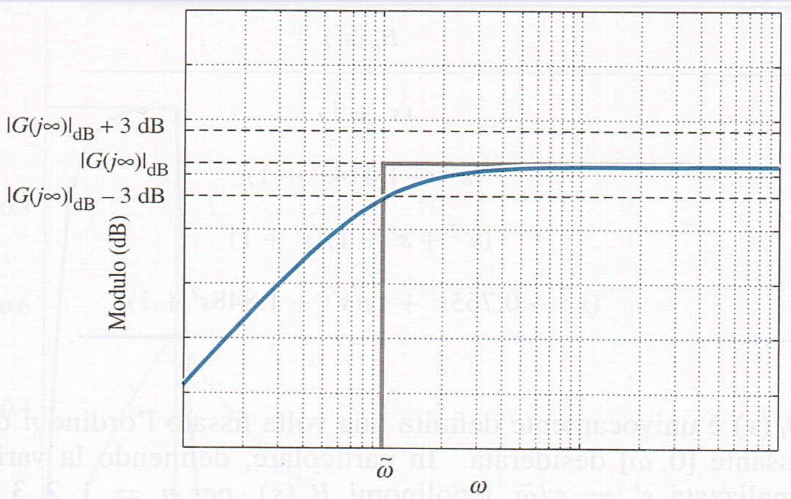
\includegraphics[width=0.5\linewidth]{immagini/screenshot003}
   			\label{fig:screenshot003}
   		\end{figure}   		
   		Anche in questo caso il filtro reale si caratterizza alla frequenza di taglio per un guadagno del 30\% inferiore, quindi sarà necessario prestare attenzione ai fattori   moltiplicativi nel suo intorno per non ottenere deamplificazioni non volute del segnale in uscita. 
   		
   		\begin{figure}[H]
   			\centering
   			\scalebox{1.5}{\begin{circuitikz}
   					%\draw [help lines] (0,0) grid (10,10);			
   					\draw (5,1) node[op amp, anchor=+] (OA1) {};    % Amplificatore
   					\draw (OA1.+) to [R, l^=$R$] (5,-0.5) node[ground]{};       % Ramo non invertente 1 a terra
   					\draw (OA1.+) to [C, l^=$C_i$] (3,1) to[european voltage source, l_=$V_i$] (3,-0.5) -- (3,-0.5) node[ground]{}; % Ramo non invertente 2 col segnale
   					\draw (OA1.-) to [R, l_=$R_i$] (2,2) -- (2,-0.5) node[ground]{}; % Ramo invertente a terra
   					\draw (OA1.-) -- (5,3) to [R, l^=$R_f$] (5,3 -| OA1.out) -- (OA1.out); % Ramo di feedback
   					\draw (7.5,1) -- (7.5,-0.5) node[ground]{$V_{out}$};	% Uscita		
   			\end{circuitikz}}
   		\end{figure}   		   		
   		Equivalentemente al filtro Passa Basso si avrà:   		
   		\begin{figure}[H]
   			\centering
   			\scalebox{0.8}{\begin{circuitikz}
   					%\draw [help lines] (0,0) grid (5,5);			
   					\draw (0,0) to[european voltage source, l^=$V_i$] (0,5) -- (3,5) to [generic, l^=$Z_C$] (3,2.5) to [generic, l^=$Z_R$] (3,1) -- (3,0) -- (0,0); % Circuito 
   					\draw (3,2.5) 	to [short, -*]	(5,2.5); 
   					\draw (3,0.5) 	to [short, -*]	(5,0.5); 
   					\draw (5,0.5)to[open,v_>=$V_+$,*-*](5,2.5);
   			\end{circuitikz}}
   		\end{figure}   		
   		Dove il partorire permette di ottenere:
   		\[V_+ = {Z_R\over Z_R + Z_C}V_i = {R\over R + {1\over j\omega C}}V_i = {j\omega RC\over 1+j\omega RC}V_i\]
   		Pertanto:
   		\[V_{out} = \left(1+{R_f\over R_i}\right)V_+ = \left(1+{R_f\over R_i}\right){j\omega RC\over 1+j\omega RC}V_i\]
   		Razionalizzando:
   		\[ V_{out} = \left(1+{R_f\over R_i}\right){\omega RC\over 1 + (\omega RC)^2} (j+\omega RC)V_i\]
   		Il guadagno sarà così: 
   		\[ G = \left(1+{R_f\over R_i}\right) {\omega RC\over \sqrt{1+(\omega RC)^2}} \]
   		Per $\omega\rightarrow0 ~~ G\rightarrow0$, per $\omega\rightarrow\infty ~~ G\rightarrow1+{R_f\over R_i}$.    		
   		\begin{figure}[H]
   			\centering
   			\begin{tikzpicture}
   				\begin{axis}[
   					axis lines = left,
   					xlabel = \(\omega\),
   					ylabel = {\(G\)},ymax=1.1,
   					xticklabels=\empty,yticklabels=\empty, extra y ticks={1}, extra y tick labels={$1+{R_f \over R_i}$}]
   					\addplot [domain=0:5, 
   					samples=100, line width=1pt
   					] {
   						(x)/((1+x^2)^(1/2))
   					};
   				\end{axis}
   			\end{tikzpicture}
   		\end{figure}   		
   		Anche in questo caso la frequenza di taglio è pari a:
   		\[-3 dB = 20\log\left(G_{f_t}\over G_0\right) \Rightarrow -3 dB = 20\log\left({\omega RC\over \sqrt{1+(\omega RC)^2}}\right)\]
   		Ovvero ci si chiede quando: 
   		\[{\omega RC\over \sqrt{1+(\omega RC)^2}} = {1\over\sqrt{2}} \Leftrightarrow \omega_{f_t} = 2\pi f_t = {1\over RC} \Rightarrow f_t = {1\over2\pi RC}\]
   		In che modo si comporta il filtro per pulsazioni e frequenze decrescenti? Se $\omega$ decresce molto il guadagno diviene: 
   		\[G = \left(1+{R_f\over R_i}\right)\omega RC\]
   		Si comporta come un circuito derivatore, ad $\omega$ minori, non oggetto del filtraggio, il segnale viene deamplificato e derivato. 
\end{adjustwidth}
\newpage
\subsection{Filtri Attivo Passa Banda}
\begin{adjustwidth}{2in}{}
   		In questo caso interessa far passare una banda mediana tra due frequenze di taglio $f_{t1}$ ed $f_{t2}$.   		
   		\begin{figure}[H]
   			\centering
   			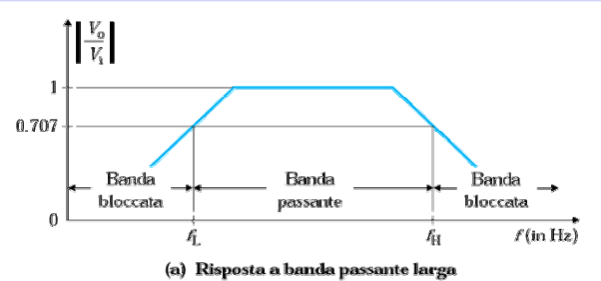
\includegraphics[width=0.5\linewidth]{immagini/screenshot004}
   			\label{fig:screenshot004}
   		\end{figure}   		  		
   		Il filtro Passa Banda può essere ad Ampia banda o a Stretta banda, che questa trattazione non tratterà. 
   		
   		disegno del guadagno preciso con dettaglio dello spettro lasciato passare
   		
   		Si definiscono: 
   		\begin{itemize}
   			\item \textbf{Frequenza Centrale} 
   			\[f_c = \sqrt{f_{bb}f_{ba}}\]
   			\item \textbf{Fattore di Forma}
   			\[Q = \dfrac{f_c}{f_{ba}-f_{bb}}\]
   		\end{itemize}
   	
   		Si sceglie perciò un filtro Passa Alto alla più bassa frequenza necessaria e un Passa Basso alla più alta frequenza necessaria:
   		\[f_{PB} = f_{ba} > f_{bb} = f_{PA}\]   		
   		\begin{figure}[H]
   			\centering
   			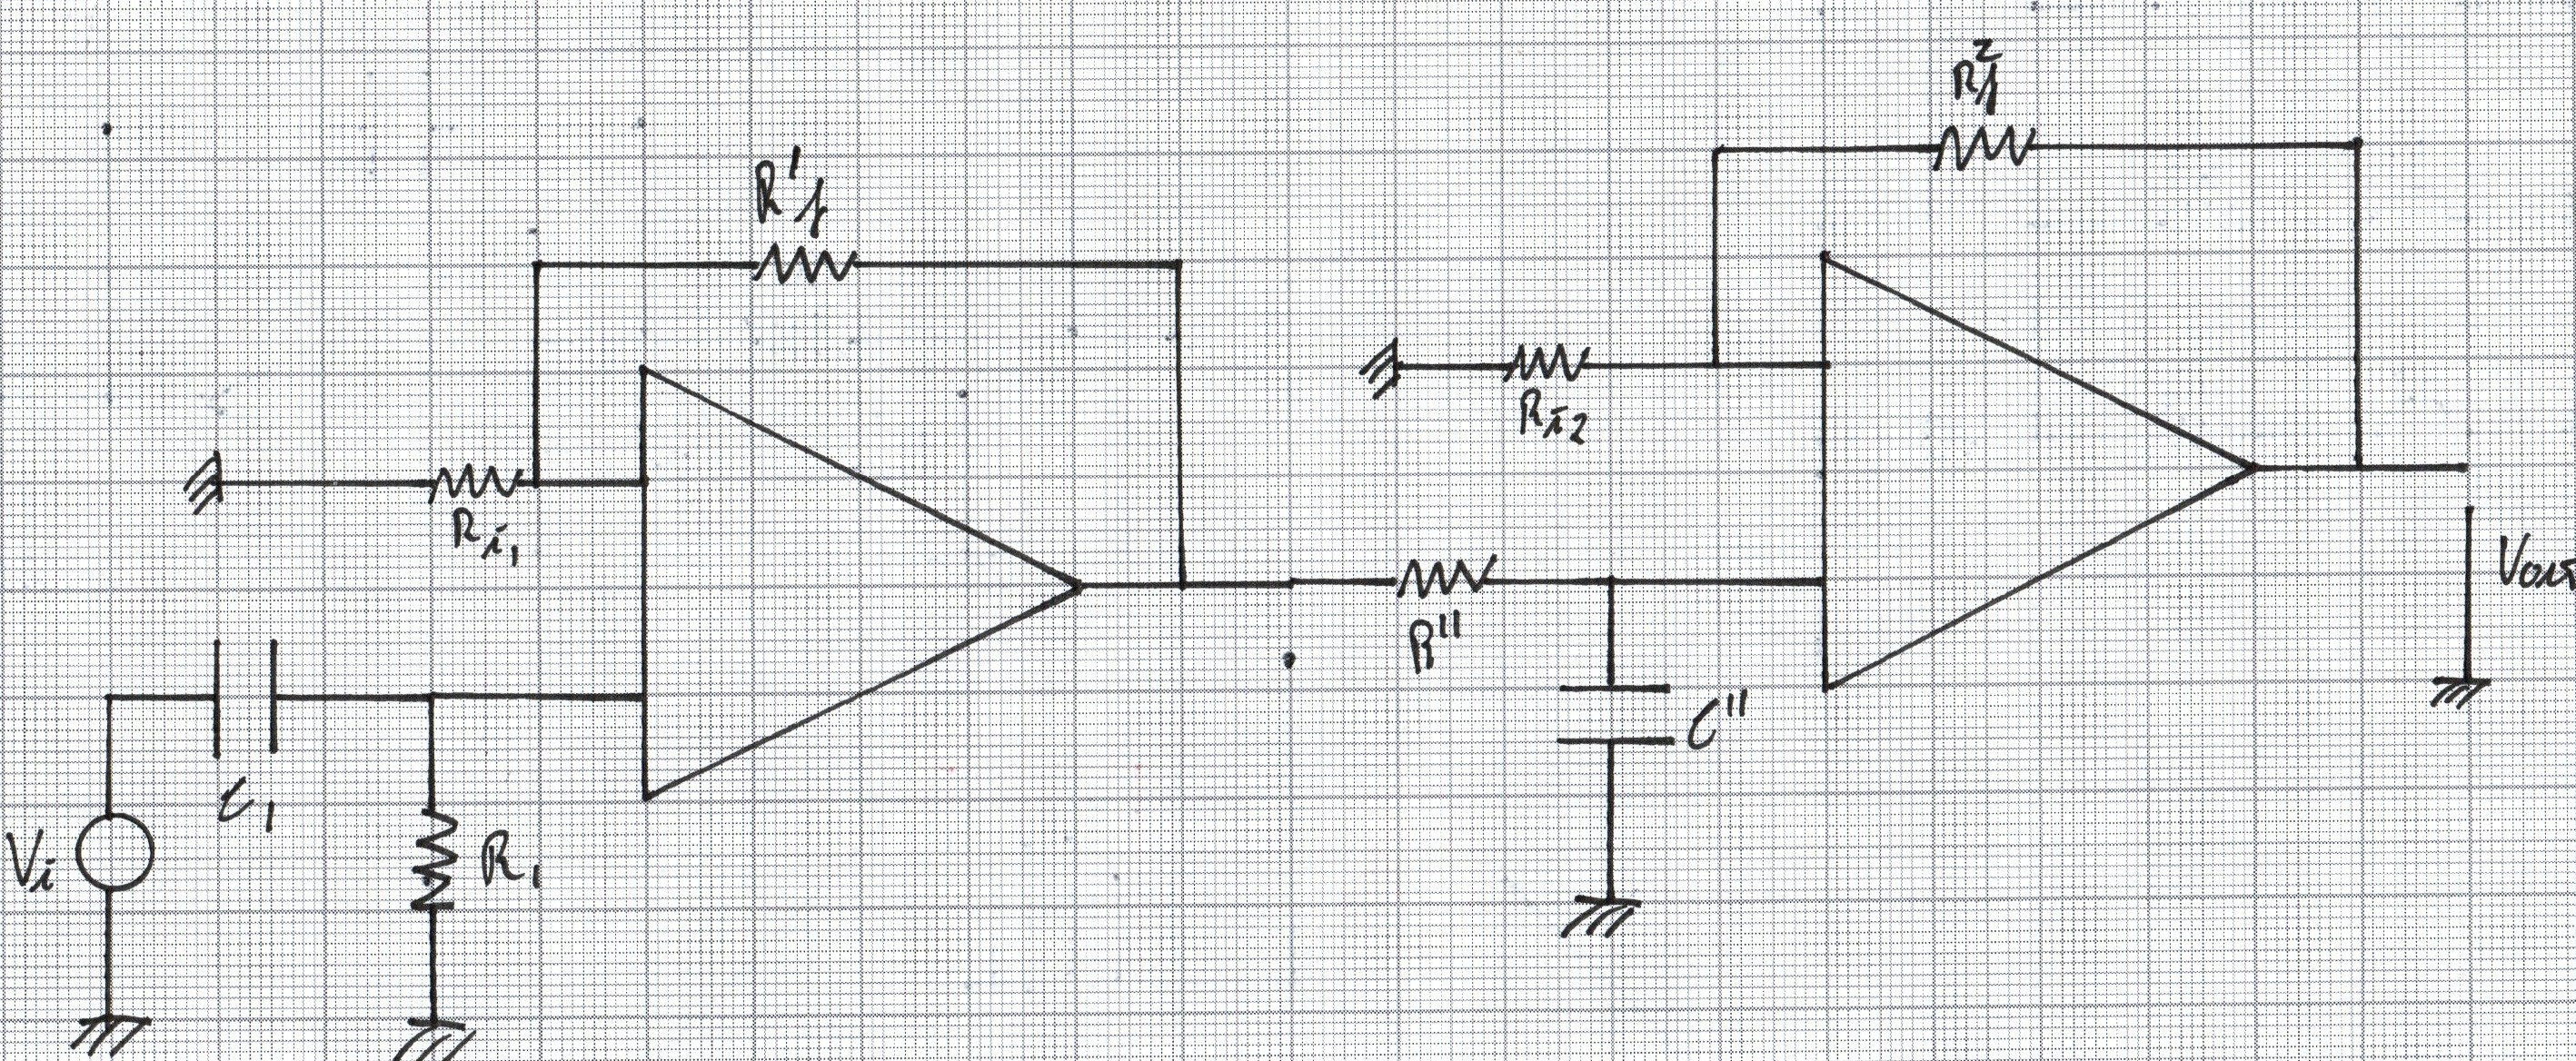
\includegraphics[width=0.5\linewidth]{immagini/mm(22)}
   			\label{fig:mm22}
   		\end{figure}   	  		
   		\[V_{out}' = \left(1+{R_f'\over R_i'}\right){j\omega R'C'\over 1+j\omega R'C'}V_i \]
   		\[V_{out} = \left(1+{R_f''\over R_i''}\right)\dfrac{1}{1+j\omega R''C''}V_{out}' \]
   		\[f_{PA} = f_{bb} = {1\over R'C'} \hspace{1cm} f_{PB} = f_{ba} = {1\over R''C''}\]
\end{adjustwidth}
\newpage
\subsection{Filtri Attivo a Reiezione di Banda o Filtro Notch}
\begin{adjustwidth}{2in}{}

   		In questo caso interessa un segnale che elimini delle frequenze mediane, si utilizza ad esempio, per eliminare il segnale a 50 Hz nell'analisi dei dati.    		
   		\begin{figure}[H]
   			\centering
   			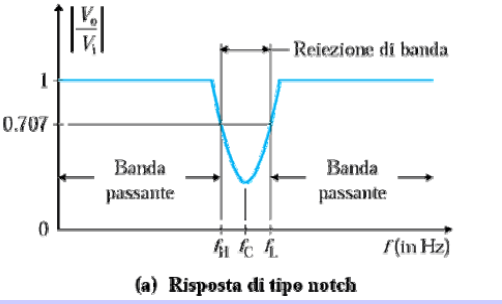
\includegraphics[width=0.5\linewidth]{immagini/screenshot005}
   			\label{fig:screenshot005}
   		\end{figure}
   		
   		\begin{figure}[H]
   			\centering
   			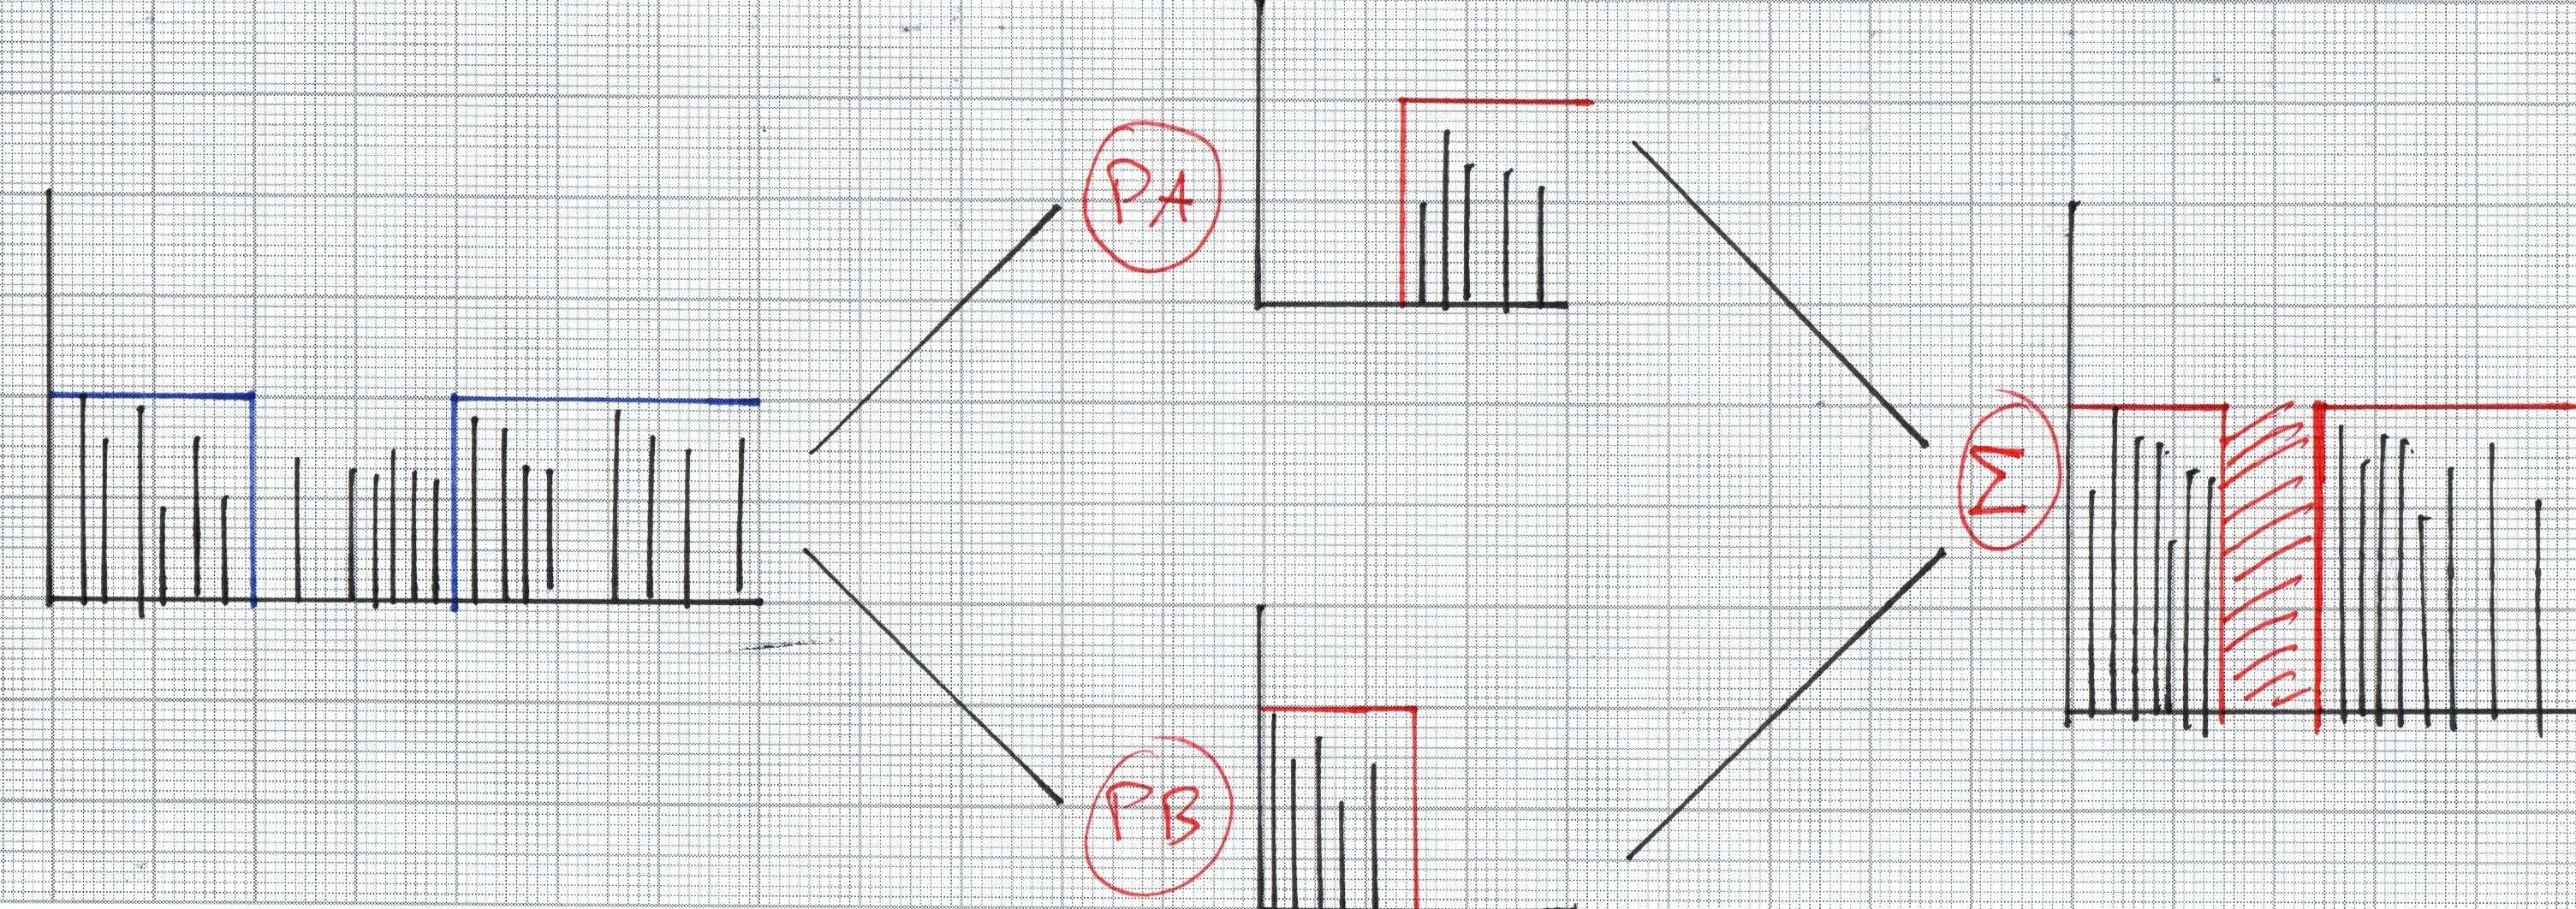
\includegraphics[width=0.5\linewidth]{immagini/mm(21)}
   			\label{fig:mm21}
   		\end{figure}   	   		
   		Si sceglie così di lavorare in parallelo con lo stesso segnale in ingresso applicandogli un filtro Passa Alto, un filtro Passa Basso e alla fine un sommatore che darà il segnale in uscita.    		
   		\begin{figure}[H]
   			\centering
   			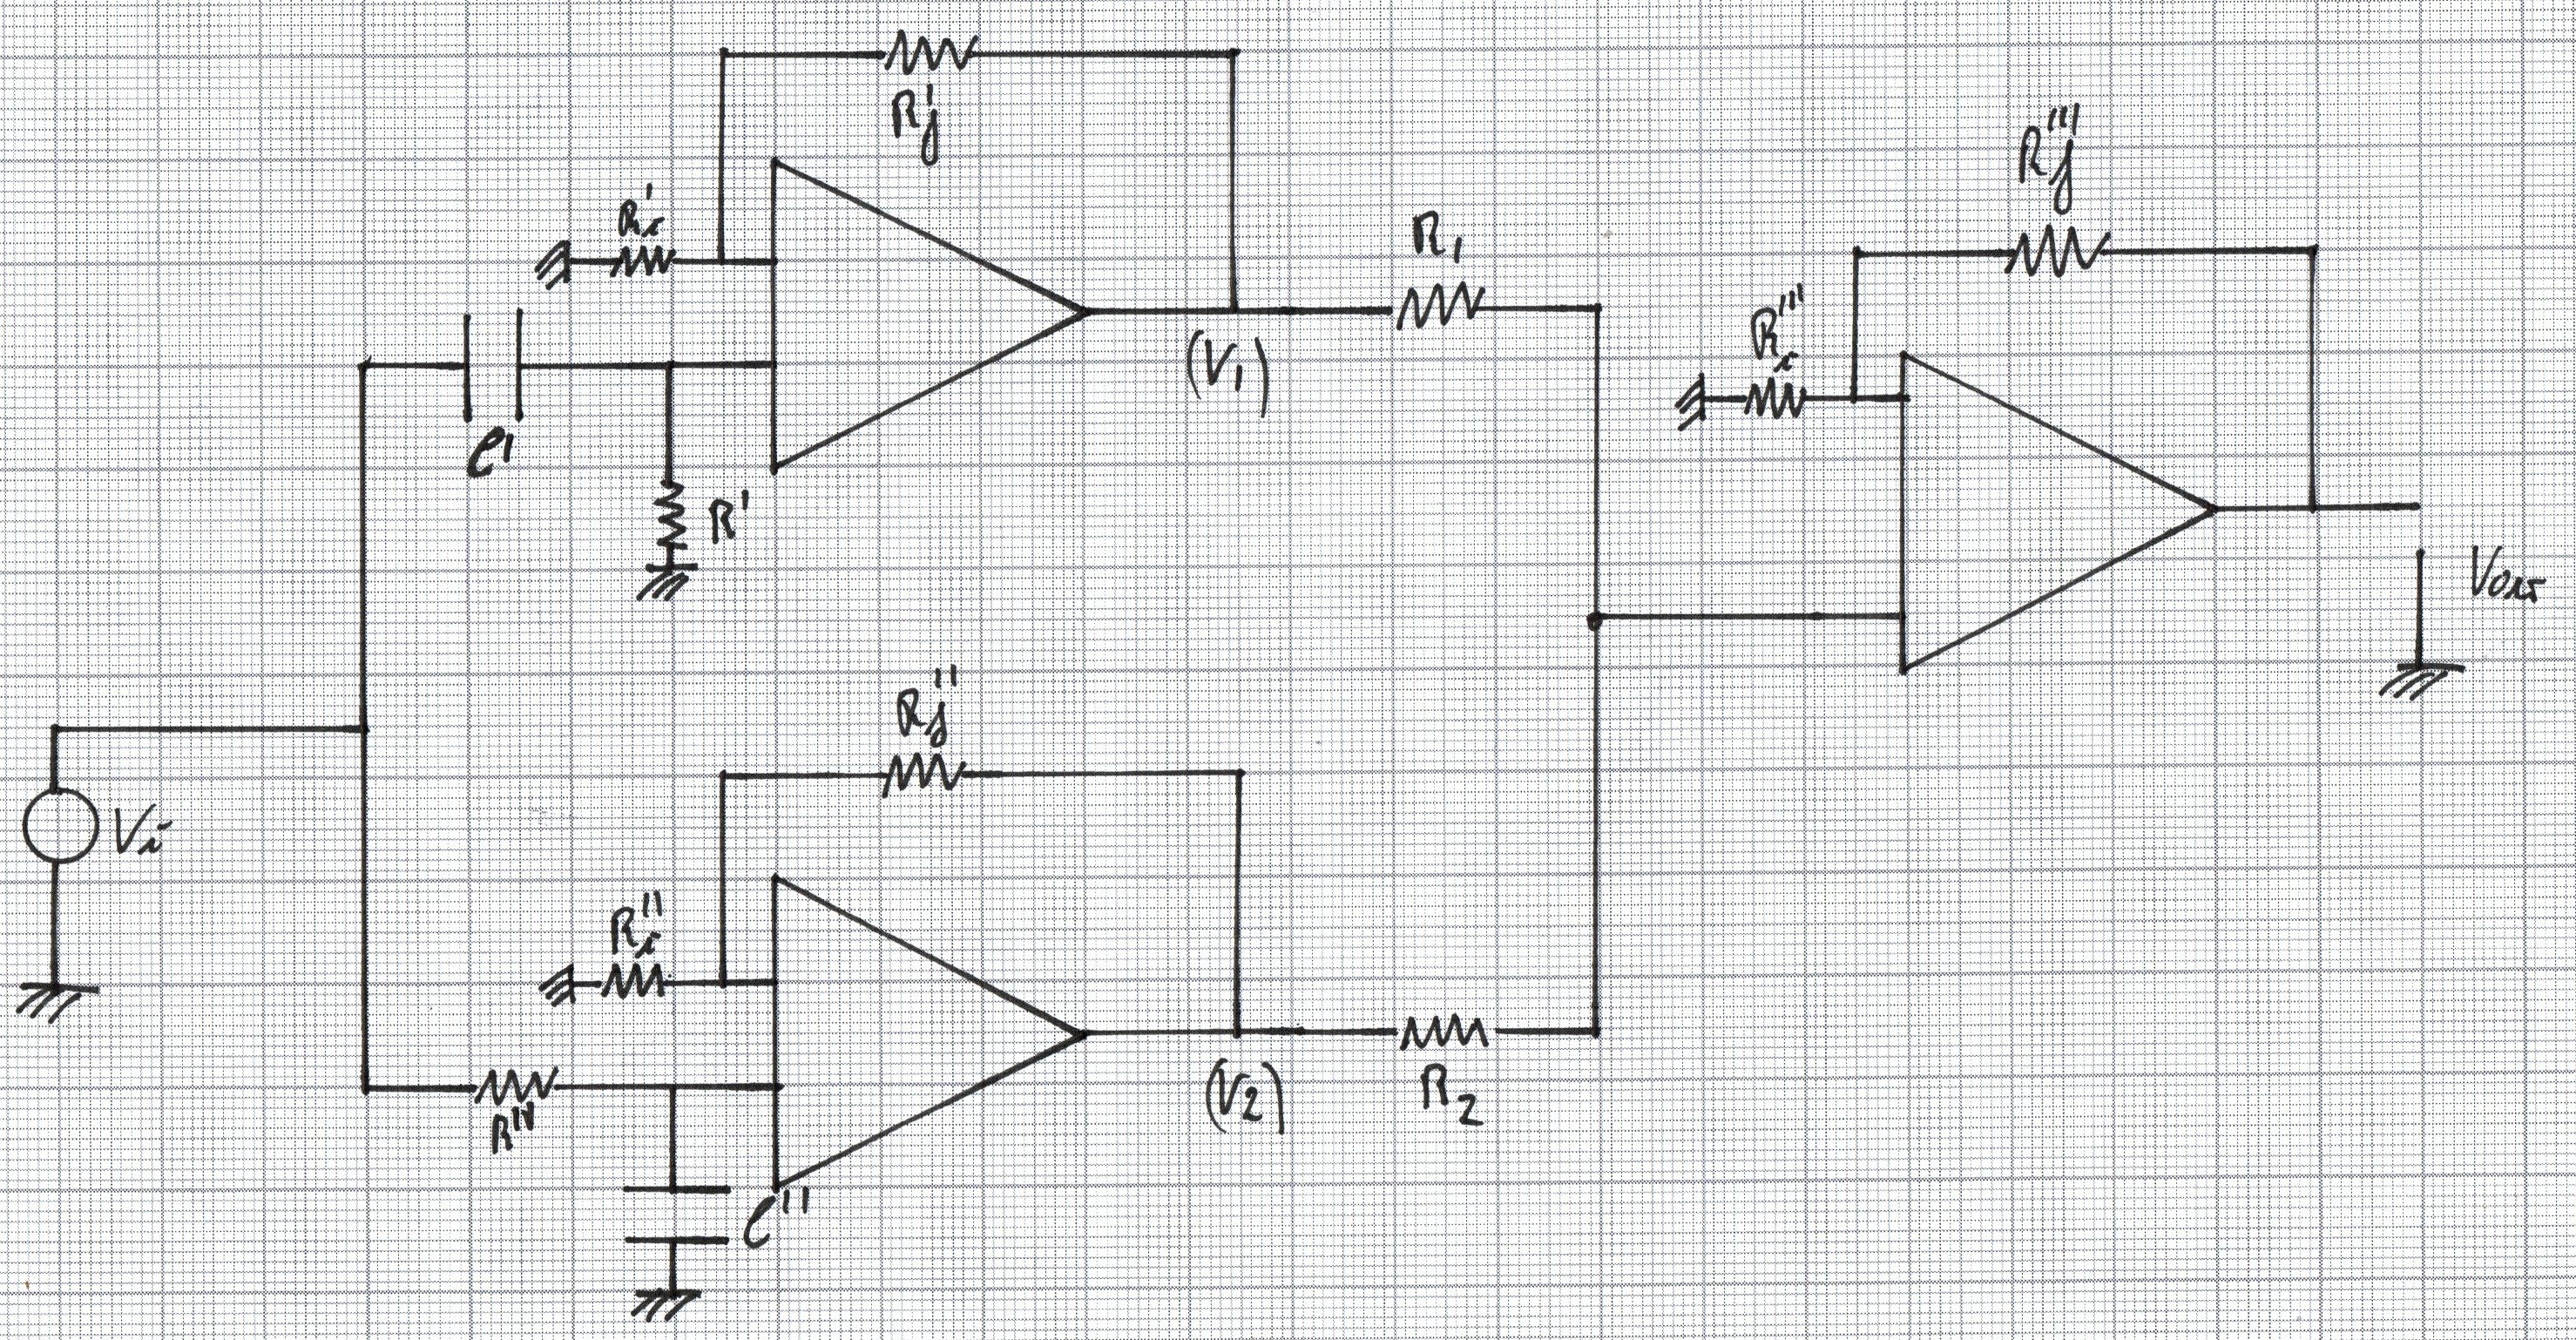
\includegraphics[width=0.5\linewidth]{immagini/mm(23)}
   			\label{fig:mm23}
   		\end{figure}   		   		
   		Per assicurarsi di avere la somma in uscita sarà necessario scegliere: $R_1 = R_2 = R_i''' = R_f'''$., in questo modo: 
   		\[V_{out} = V_1 + V_2 = \left(1+{R_f'\over R_i'}\right){j\omega R'C'\over 1+j\omega R'C'}V_i + \left(1+{R_f''\over R_i''}\right)\dfrac{1}{1+j\omega R''C''}V_{out}' \]
   		Si sceglie perciò un filtro Passa Alto alla minore delle maggiori frequenze necessarie per filtrare le  alte frequenze e un Passa Basso alla più alta delle minori frequenze necessarie per filtrare le basse frequenze:
   		\[f_{PB} = f_{bb} < f_{ba} = f_{PA}\]
   		\[f_{PB} = f_{bb} = {1\over R''C''} \hspace{1cm} f_{PA} = f_{ba} = {1\over R'C'}\]
   		
\newpage

{\LARGE \textbf{NOTE}}
	
	%DA DECOMMENTARE PER AVERE LA VERSIONE STAMPABILE A DUE PAGINE 	
	%	\newpage
	%		\null
	%		\vfill
	%\begin{tcolorbox}[height=4.5cm]
	%	This box has a height of 4.5cm.
	%\end{tcolorbox}
	%		
\end{adjustwidth}
\end{document}